% !TEX encoding = UTF-8 Unicode
% !BIB TS-program = biber 
%%%%%%%%%%%%%%%%%%%%%%%%%%%%%%%%%%%%%%%

\documentclass[twoside,fontset=newtx-sans-text]{mitthesis}

\usepackage[spanish]{babel}
\usepackage{amsmath,amssymb,amsfonts}		
\usepackage{listings}
\usepackage{booktabs}
\usepackage{array}
\usepackage{pdfpages}

\newtheorem{notation}{Notación}[chapter]
\newtheorem{theorem}{Teorema}[chapter]
\newtheorem{definition}{Definición}[chapter]
\newtheorem{lemma}{Lema}[chapter]
%% Set chemical formulas nicely
% \usepackage[version=4]{mhchem}%   documentation is here https://ctan.org/pkg/mhchem
\graphicspath{{assets/}}
\usepackage{csquotes} 

\usepackage[
    style=apa,
    sortcites=true,
    sorting=nyt,
    backend=biber,
    language=spanish,
    hyperref=true,
    backref=true,
]{biblatex}

\addbibresource{bibliography.bib}

\hypersetup{
	pdfsubject={Ecuaciones de Navier-Stokes},
	pdfkeywords={Universidad Autónoma Chapingo, UACh},
	pdfurl={},
	pdfcontactemail={emilioah02@gmail.com},
	pdfauthortitle={Ing.}
}

\pagestyle{plain}

\def\all{all}
\ifx\files\all \typeout{Including all files.} \else %\typeout{Including only \files.} \includeonly{\files} \fi

% Márgenes
\geometry{left=4cm, right=2.5cm, top=5cm, bottom=2.5cm}

\begin{document}

\title{DESARROLLO DE UNA APLICACIÓN MULTIPLATAFORMA BASADA EN CIENCIA CIUDADANA PARA EL MONITOREO DE LLUVIA EN EL MONTE TLÁLOC}
\Author{LUIS EMILIO ÁLVAREZ HERRERA}{Departamento de Irrigación}
\Degree{INGENIERO EN IRRIGACIÓN}{DEPARTAMENTO DE IRRIGACIÓN}
\Supervisor{Dra. Teresa Margarita Gonzalez Martínez}{Profesora del COLPOS}
\Supervisor{Luis Tonatiuh Castellanos Serrano}{Profesor del DIMA}
\Supervisor{Francisco García Herrera}{Profesor de Irrigación}
\Supervisor{Ramón Arteaga Ramírez}{Profesor de Irrigación}
\Supervisor{Bernardino Cruz}{Profesor de Irrigación}
\DegreeDate{June}{2025}
\ThesisDate{June 15, 2025}
\CClicense{CC BY-NC-ND 4.0}{https://creativecommons.org/licenses/by-nc-nd/4.0/}

%%%%%%% INICIA NÚMEROS ROMANOS %%%%%%%

 

\includepdf[pages=1]{0cover.pdf}
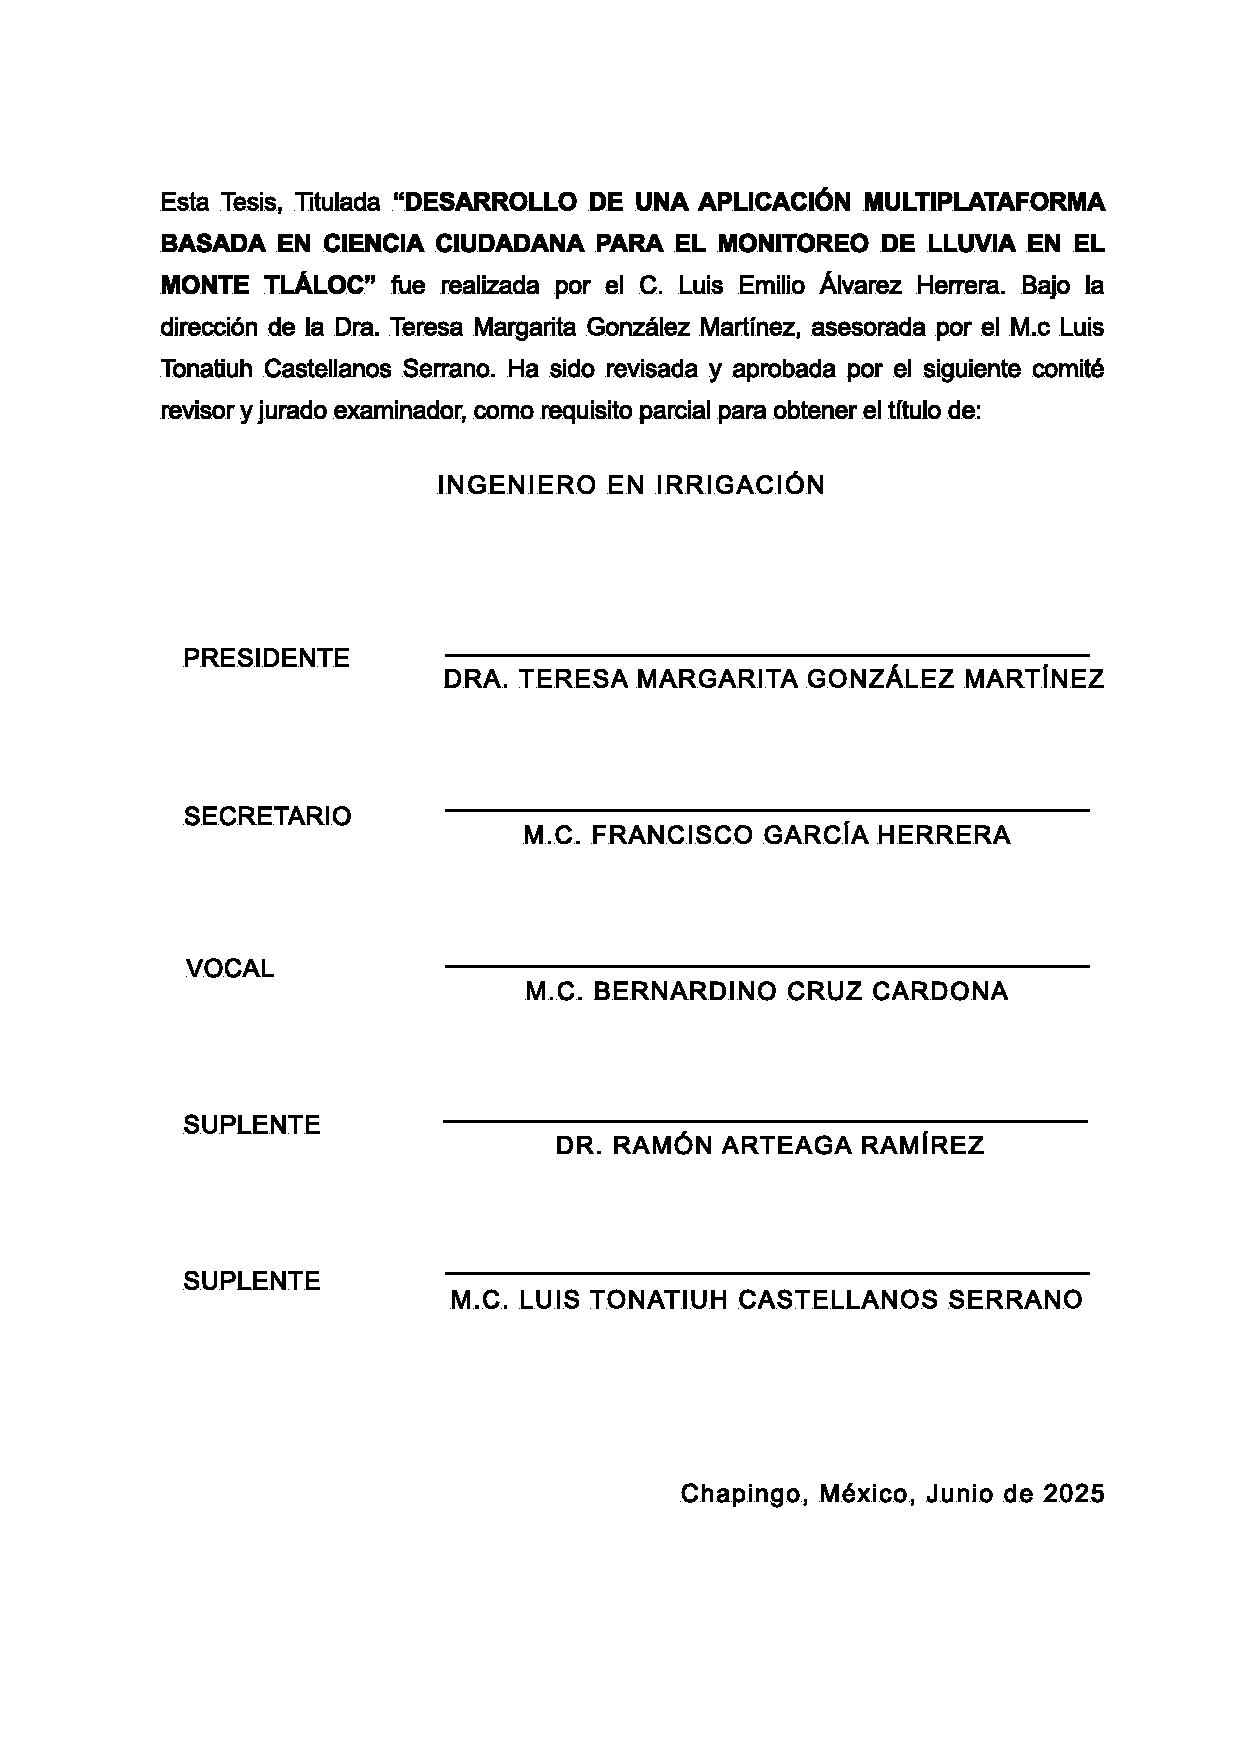
\includepdf[pages=1]{01sign.pdf}

\pagenumbering{roman}


\chapter*{AGRADECIMIENTOS}
\addcontentsline{toc}{chapter}{AGRADECIMIENTOS}
\begin{center}
    \texttt{``La educación agrícola es la base para una nación fuerte y autosuficiente''} - Marte R. Gómez, padre de la Universidad Autónoma Chapingo, ingeniero hidráulico.
\end{center}

Hago especial reconocimiento por las enseñanzas y valores que adquirí gracias a la \textbf{Universidad Autónoma Chapingo}: por ofrecerme la beca institucional, por la beca PROFONI referente a la investigación; por la beca SUBES y Benito Juárez del gobierno de México; al Comedor Central y Unidad Médica por su servicio de primera calidad; en especial estoy agradecido a causa de toda la inversión por concepto de:
\begin{itemize}
    \item Congreso Internacional en Santiago Chile, 
    \item Intercambio Académico Internacional que fue en la Universidad de Agricultura de Tokio, 
    \item por la estancia preprofesional en EcosueloLab Chile, 
    \item Viajes de estudio en México
    \item y por sus numerosos vínculos con instituciones prestigiosas, especialmente con el Colegio de Posgraduados de donde surgió este trabajo.
\end{itemize}

Hago un distinguido reconocimiento a las y los maestros que me han enseñaron desde el kínder hasta la universidad, todos ellos merecen nuestro profundo respeto, admiración y gratitud. Además, es honorable el trabajo físico y arduo que realiza el personal administrativo o plantilla de trabajadores por mantener en funcionamiento las instalaciones.

Finalmente al \textbf{Proyecto Miyotl}, una app para preservar, difundir y enseñar las lenguas mexicanas para los pueblos indígenas.
\newpage

\chapter*{DEDICATORIA}
\addcontentsline{toc}{chapter}{AGRADECIMIENTOS}

A mi mamá \texttt{María Carolina Herrera Díaz} y a mi papá Agustín Álvarez Bautista, cuyos sacrificios y amor incondicional me han dado la fortaleza para alcanzar mis metas. Ustedes me enseñaron que la educación es el legado más valioso y que el esfuerzo constante siempre rinde frutos. Cada paso que doy es un reflejo de su dedicación y valores inculcados. 

A mis abuelos Laura Díaz Cruz - Mamá Aya, Mario Herrera Munguía - Papá Gogo$^\dag$, Luisa y Agustín, guardianes de la sabiduría y el cariño eterno. Aunque algunos ya no estén físicamente, sus enseñanzas y amor permanecen vivos en mi corazón. Sus historias y consejos me han guiado en los momentos más difíciles, dándome el coraje para persistir y superar obstáculos.

A mis hermanos Paulo Elías Fernández Herrera, Alan Yareth Álvarez Zarco y Aranza Ailín Álvarez Zarco, incondicionales de aventuras y desafíos. Gracias por ser mi apoyo en los días grises y mi celebración en los días de triunfo. Su confianza en mí ha sido una fuente de motivación constante.

A mis maestros Humberto López Chimil$^\dag$, Fernando Chávez León$^\dag$; a mis mentores Luis Tonatiuh Castellanos Serrano, la Dra. Teresa González Martínez, que con su sabiduría y paciencia han encendido en mí la llama del conocimiento. Sus enseñanzas han trascendido las aulas y han dejado una huella imborrable en mi formación personal y profesional. Gracias por creer en mi potencial y por inspirarme a ser mejor cada día.

A la Universidad Autónoma Chapingo y al Departamento de Irrigación que me llevaron tan lejos como a Sudamérica, Asia y a lo largo y ancho del mejor país del mundo: \textbf{México}.

Finalmente, dedico esta tesis a Dios, porque el me dio la voluntad de perseverar a pesar de las adversidades, por cada noche en vela y cada instante de duda superado. Este logro es el resultado de años de esfuerzo y dedicación, me recuerda que los sueños se alcanzan con determinación y pasión. Gracias a todos los que han sido parte de este viaje. Esta tesis es una manifestación de tu amor, apoyo y fe en mí.

%% biography.tex
%% This section is optional

% From mitthesis package
% Version: 1.01, 2023/10/16
% Documentation: https://ctan.org/pkg/mitthesis

% \chapter*{DATOS BIOGRÁFICOS}
% \addcontentsline{toc}{chapter}{DATOS BIOGRÁFICOS}

% \textbf{Luis Emilio Álvarez Herrera} nació el 7 de junio de 2002 en Texcoco de Mora, estado de México. Ingresó a la Universidad Autónoma Chapingo en 2017 y se incorporó al Departamento de Irrigación en 2020.

% Durante su formación académica, realizó un intercambio en la Universidad de Agricultura de Tokio, Japón (2023) y efectuó sus prácticas profesionales en Ecosuelo Lab, Santiago Chile (2025).

% Fue miembro del Programa de Formación de Nuevos Investigadores (PROFONI) de 2021 a 2025. 

% Es autor de tres libros: \textit{Fundamentos de la Ingeniería en Irrigación} (ocho volúmenes), \textit{Matemáticas del Cubo Rubik} y \textit{Huertos Agroecológicos}.

% Entre 2017 y 2022, se dedicó a la docencia de matemáticas en el Colegio Euro Texcoco, como asistente del maestro Fernando Chávez León. 

% Se desempeñó como consejero departamental de la Preparatoria Agrícola en 2018; en 2020, nuevamente fue consejero, ahora en el Departamento de Irrigación; Y como presidente del Club de Ciencias Netzahualpilli de 2019 a 2022. 

% Actualmente, es CEO del proyecto \textit{Miyotl: Aprende una lengua indígena}, CTO de \textit{Tláloc App: Ciencia ciudadana para el monitoreo de lluvia en el Monte Tláloc} (COLPOS) y CEO de la \textit{Olimpiada Mexicana de Agronomía}.





\renewcommand{\contentsname}{CONTENIDO}
\tableofcontents

\renewcommand{\listtablename}{LISTA DE CUADROS}
\listoftables

\renewcommand{\listfigurename}{LISTA DE FIGURAS}
\listoffigures

\renewcommand{\abstractname}{RESUMEN}
% From mitthesis package
% Version: 1.01, 2023/06/19
% Documentation: https://ctan.org/pkg/mitthesis
%
% The abstract environment creates all the required headers and footnote. 
% You only need to add the text of the abstract itself.
%
% Approximately 500 words or less; try not to use formulas or special characters
% If you don't want an initial indentation, do \noindent at the start of the abstract
\begin{abstract}
% use \input rather than \include because we're inside an environment

Recientes esfuerzos en ciencia ciudadana han demostrado el valor de las aplicaciones móviles para el monitoreo ambiental distribuido. En esta tesis, se presenta el desarrollo de Tláloc App, una aplicación multiplataforma basada en Flutter, diseñada para registrar y analizar datos de precipitación pluvial en el Monte Tláloc, utilizando la participación activa de los usuarios. La plataforma integra tecnologías como Firebase Realtime Database para almacenamiento en tiempo real, Google Play Console para su despliegue en Android, y algoritmos personalizados para el cálculo de mediciones reales basadas en el estado de vaciado de pluviómetros. El enfoque modular de desarrollo incluye una experiencia de usuario adaptable y escalable. Los resultados obtenidos demuestran que Tláloc App facilita la recolección sistemática de datos meteorológicos de forma económica y participativa, con posibilidades de expansión a otras regiones. Esta investigación propone un nuevo modelo de colaboración entre ciencia ciudadana y tecnología móvil en entornos de alta variabilidad climática.



\textbf{Palabras-Clave:} Ciencia ciudadana, monitoreo de lluvia, Aplicaciones móviles.
\end{abstract}

\renewcommand\abstractname{ABSTRACT}
\begin{abstract}
	Recent efforts in citizen science have demonstrated the value of mobile applications for distributed environmental monitoring. This thesis presents the development of Tláloc App, a cross-platform application built with Flutter, designed to record and analyze rainfall data at Monte Tláloc through active user participation. The platform integrates technologies such as Firebase Realtime Database for real-time data storage, Google Play Console for Android deployment, and custom algorithms for calculating real measurements based on rain gauge statuses. The modular development approach includes a scalable and adaptable user experience. Results show that Tláloc App enables systematic, low-cost, and participatory meteorological data collection, with potential expansion to other regions. This research proposes a new model of collaboration between citizen science and mobile technology in areas with high climatic variability.


	
\textbf{Key-Words:} Citizen science, Rainfall monitoring, Mobile application
\end{abstract}

 
%%%%%% CAMBIAR A NÚMEROS ARÁBIGOS DESPUÉS DE FRONTAL %%%%%%%

\clearpage
\pagenumbering{arabic}

\newgeometry{left=4cm, right=2.5cm, top=2.5cm, bottom=2.5cm, marginparwidth=0pt, headsep=0pt}
\chapter{INTRODUCCIÓN}
\pagenumbering{arabic}
\setcounter{page}{1}

Las montañas actúan como barreras orográficas que obligan a las nubes a elevarse y enfriarse, lo que genera precipitaciones más abundantes en comparación con los valles circundantes. Sin embargo, la medición de estas lluvias en zonas montañosas suele ser limitada debido a su difícil acceso y a la falta de vigilancia para el mantenimiento de instrumentos de medición (\cite{aparicio1992}). Esta situación es crítica en ecosistemas como los bosques, donde la información sobre precipitación resulta fundamental para su conservación y manejo. Los bosques templados de montaña, como los del Monte Tláloc en México, enfrentan múltiples desafíos, entre ellos la deforestación, la fragmentación del hábitat y los efectos del cambio climático. Este último ha generado alteraciones en los patrones de precipitación y temperatura, impactando negativamente la biodiversidad, los ciclos hidrológicos y los servicios ecosistémicos que estos bosques proporcionan (\cite{gonzalez2016}).

Actualmente el ejido tiene participación en los programas forestales con 1628 hectáreas de superficie forestal en Monte Tláloc y ante la CONAFOR se tienen registradas 248 hectáreas para aprovechamiento forestal (\cite{nava2014}). Según (\cite{lopez2023}), en el Monte Tláloc, las extracciones por nivel altitudinal parecen estar relacionadas con la elevada mortalidad de árboles en las categorías más pequeñas, sin embargo, la intensidad y nivel de extracción de madera no parecen representar una amenaza que ponga en riesgo la viabilidad poblacional de Abies religiosa; la categoría diamétrica más pequeña parece beneficiarse de las aperturas debidas a las extracciones. El cambio climático repercute de diferente manera en el crecimiento de los bosques de montaña en los extremos altitudinales de su distribución; así como su relación con el proceso de migración de fauna, y finalmente los ecosistemas terminan siendo amenazados \cite{hernandez2021}.

El objetivo principal de este estudio es desarrollar una aplicación móvil y web que facilite el monitoreo de la precipitación en el Monte Tláloc mediante la participación activa de ejidatarios y otros grupos de interés. A través de esta herramienta tecnológica, se busca implementar una estrategia de ciencia ciudadana que permita registrar, analizar y visualizar datos de lluvia, contribuyendo así a la gestión sostenible de los recursos naturales y la conservación de los bosques de montaña.

\section{Planteamiento del problema}

Ante la falta de datos sobre precipitación en estas zonas, se requiere el desarrollo de estrategias innovadoras que permitan superar las limitaciones técnicas y logísticas, involucrando a las comunidades locales en la generación y uso de información. Es necesario recurrir a estrategias que incorporen a la población en la generación de información y en su utilización para el manejo de los ecosistemas \cite{hubp1990}.

En México, las redes oficiales de monitoreo hidrometeorológico, como las operadas por la Comisión Nacional del Agua (CONAGUA), presentan una cobertura limitada en muchas regiones de montaña, donde los microclimas pueden variar significativamente en distancias cortas.

El Monte Tláloc, ubicado en la zona montañosa del oriente del Valle de México, es un ejemplo de ello: su importancia ambiental, histórica y cultural contrasta con la escasa información climática precisa y en tiempo real disponible para la comunidad local, investigadores y tomadores de decisiones. Esta falta de datos puntuales dificulta la \textbf{gestión sustentable del agua}, la prevención de riesgos y el análisis del cambio climático a escala local.

Las aplicaciones disponibles para la recolección de datos meteorológicos suelen ser de uso profesional, poco accesibles o no están diseñadas para fomentar la participación ciudadana en contextos rurales o de baja conectividad. Esto genera una brecha entre el potencial de colaboración ciudadana y las herramientas disponibles para lograrlo.

Ante este panorama, surge la necesidad de desarrollar una aplicación multiplataforma intuitiva, accesible y robusta, que aproveche el poder de la ciencia ciudadana para llenar los vacíos de información sobre la precipitación en el Monte Tláloc. Dicha aplicación debe facilitar la recolección, visualización y validación de datos por parte de usuarios no expertos, promoviendo la generación de conocimiento colectivo, la educación ambiental y la participación activa de la comunidad en temas de gestión hídrica y climática.


\section{Planteamiento del problema}

Ante la falta de datos sobre precipitación en estas zonas, se requiere el desarrollo de estrategias innovadoras que permitan superar las limitaciones técnicas y logísticas, involucrando a las comunidades locales en la generación y uso de información. Es necesario recurrir a estrategias que incorporen a la población en la generación de información y en su utilización para el manejo de los ecosistemas (\cite{hubp1990}).


En México, las redes oficiales de monitoreo hidrometeorológico, como las operadas por la Comisión Nacional del Agua (CONAGUA), presentan una cobertura limitada en muchas regiones de montaña, donde los microclimas pueden variar significativamente en distancias cortas \cite{rosas2021}. 


El Monte Tláloc, ubicado en la zona montañosa del oriente del Valle de México, es un ejemplo de ello: su importancia ambiental, histórica y cultural contrasta con la escasa información climática precisa y en tiempo real disponible para la comunidad local, investigadores y tomadores de decisiones. Esta falta de datos puntuales dificulta la \textbf{gestión sustentable del agua}, la prevención de riesgos y el análisis del cambio climático a escala local.

Las aplicaciones disponibles para la recolección de datos meteorológicos suelen ser de uso profesional, poco accesibles o no están diseñadas para fomentar la participación ciudadana en contextos rurales o de baja conectividad. Esto genera una brecha entre el potencial de colaboración ciudadana y las herramientas disponibles para lograrlo.

Ante este panorama, surge la necesidad de desarrollar una aplicación multiplataforma intuitiva, accesible y robusta, que aproveche el poder de la ciencia ciudadana para llenar los vacíos de información sobre la precipitación en el Monte Tláloc. Dicha aplicación debe facilitar la recolección, visualización y validación de datos por parte de usuarios no expertos, promoviendo la generación de conocimiento colectivo, la educación ambiental y la participación activa de la comunidad en temas de gestión hídrica y climática.



\section{Justificación}


La ciencia ciudadana surge como una alternativa viable para enfrentar esta problemática, al involucrar a la población en la recopilación de datos y en la búsqueda de soluciones. A través de herramientas tecnológicas, como aplicaciones móviles y plataformas digitales, se facilita la recolección de información de manera accesible, eficiente y en tiempo real, promoviendo a su vez la educación ambiental y la colaboración social. Esta metodología no solo proporciona datos científicos valiosos, sino que también fortalece el vínculo entre la sociedad y la conservación de los ecosistemas.

Se identifica la necesidad de crear un instrumento para la captura y envío de datos pluviales que sea accesible, participativo y que garantice la disponibilidad de la información obtenida para su análisis y toma de decisiones. Este instrumento debe ser sencillo de usar y estar diseñado específicamente para el público objetivo: los ejidatarios. Ellos, a través de su conocimiento del territorio y participación activa, pueden convertirse en aliados estratégicos para la recolección continua y precisa de datos.

La aplicación desarrollada se plantea como una solución innovadora que responde a esta necesidad. Su diseño intuitivo permite que usuarios con conocimientos tecnológicos básicos puedan capturar y enviar información sobre las precipitaciones de manera rápida y eficiente. Además, al integrar elementos de ciencia ciudadana, se fomenta la colaboración activa de las comunidades locales, fortaleciendo su empoderamiento y compromiso con la conservación de los recursos hídricos.

Desde un enfoque técnico, el proyecto destaca por su carácter práctico y adaptable. La app aprovecha tecnologías modernas para registrar datos de lluvia, optimizando la recopilación de información en tiempo real, y reduciendo costos asociados a equipos de medición tradicionales. Al centralizar y analizar estos datos en una plataforma digital, se genera un repositorio de información confiable que puede ser utilizado por investigadores, autoridades locales y los mismos ejidatarios para tomar decisiones fundamentadas. 

Por último, la disponibilidad de esta información en un formato accesible y visualmente comprensible contribuye a sensibilizar a los usuarios sobre la importancia de monitorear los patrones de lluvia, facilitando su uso en estrategias de manejo hídrico, planificación agrícola y mitigación de riesgos climáticos. De esta forma, el proyecto no solo soluciona un problema técnico, sino que también tiene un impacto social y ambiental significativo.


\section{Hipótesis}
\subsection{Hipótesis general (H)}

La implementación de una aplicación multiplataforma basada en ciencia ciudadana incrementa significativamente la frecuencia y precisión de los reportes de lluvia en la región del Monte Tláloc, al promover la participación activa de los habitantes locales mediante herramientas digitales accesibles. Esto permite generar información meteorológica complementaria a la de las estaciones profesionales, mejorando la caracterización espacial y temporal de los eventos de precipitación.


\subsection{Hipótesis nula (H0)}
La implementación de una aplicación multiplataforma basada en ciencia ciudadana \textbf{no tiene un efecto significativo} en la frecuencia ni en la precisión de los reportes de lluvia en la región del Monte Tláloc, ni contribuye sustancialmente a la caracterización de los eventos de precipitación.

\subsection{Hipótesis alternativa (H1)}
La implementación de una aplicación multiplataforma basada en ciencia ciudadana \textbf{sí mejora significativamente} la frecuencia y precisión de los reportes de lluvia en la región del Monte Tláloc, y contribuye a una mejor caracterización de los eventos de precipitación respecto a los datos generados únicamente por estaciones profesionales.











\section{Contribuciones de este trabajo}

Este trabajo de tesis contribuye al campo del desarrollo tecnológico, la ciencia ciudadana y la meteorología local mediante la creación de una aplicación multiplataforma diseñada específicamente para el monitoreo participativo de lluvia en el Monte Tláloc. La solución propuesta integra tecnologías móviles modernas con servicios en la nube y diseño centrado en el usuario, permitiendo que cualquier ciudadano pueda registrar datos de precipitación de manera sencilla, segura y estructurada. Esta contribución tiene un impacto directo en la generación de datos alternativos en regiones donde la infraestructura meteorológica es escasa o limitada, y donde los fenómenos hidrometeorológicos presentan comportamientos complejos.

Desde el punto de vista técnico, la tesis presenta una arquitectura modular desarrollada con Flutter, integrando funcionalidades clave como, sincronización con Firebase, visualización gráfica de estadísticas y un sistema para validar la veracidad de las mediciones con base en algoritmos desarrollados para la interpretación de datos de pluviómetros caseros. Se propone también una metodología de evaluación del nivel de maduración tecnológica (TRL) aplicada a aplicaciones de ciencia ciudadana, lo cual permite medir de forma objetiva el avance y aplicabilidad real del sistema desarrollado.

Además, este trabajo representa un esfuerzo por brindar el acceso a las tecnologías de monitoreo ambiental, empoderando a las comunidades rurales al integrarlas como agentes activos en la recolección de datos climáticos, al tiempo que fortalece los vínculos entre el conocimiento científico y la sabiduría local. Finalmente, se generan aportes a futuras investigaciones en temas relacionados con aplicaciones móviles para monitoreo ambiental, ciencia abierta y educación en contextos rurales, abriendo camino a iniciativas de colaboración interdisciplinaria entre desarrolladores, científicos, comunidades y tomadores de decisiones.












\section{Esquema de la tesis}

Este trabajo está estructurado de acuerdo con el proceso de investigación, desarrollo y validación de una aplicación multiplataforma basada en ciencia ciudadana para el monitoreo de lluvia en el Monte Tláloc. La introducción presenta el contexto y motivaciones del estudio, seguida de cinco capítulos que describen el planteamiento del problema, la metodología empleada, los resultados obtenidos y las conclusiones alcanzadas. La notación es consistente a lo largo del documento, y cualquier excepción está claramente indicada. La bibliografía acumulativa se presenta al final. A continuación, se ofrece una breve descripción de los capítulos.





\begin{itemize}
    \item \textbf{Capítulo 1: Introducción} Presenta el planteamiento del problema, el contexto geográfico del Monte Tláloc, la justificación del proyecto, la hipótesis de trabajo, las principales contribuciones de la tesis, el esquema general del documento y las limitaciones del estudio.
    
    \item \textbf{Capítulo 2: Objetivos} Define el objetivo general y los objetivos específicos que guiaron la realización de este trabajo de investigación y desarrollo tecnológico.
    
    \item \textbf{Capítulo 3: Revisión de literatura} Revisa los conceptos clave necesarios para entender el proyecto, incluyendo el acceso a datos meteorológicos de zonas de montaña en México, estudios previos sobre monitoreo ciudadano, tecnologías actuales en monitoreo climático, y los aportes de la ciencia ciudadana al estudio climático.
    
    \item \textbf{Capítulo 4: Materiales y Métodos} Describe los materiales físicos utilizados, la infraestructura tecnológica virtual implementada, el protocolo de monitoreo participativo, el proceso de desarrollo de la aplicación Tláloc App, y la metodología empleada para evaluar su nivel de maduración tecnológica.
    
    \item \textbf{Capítulo 5: Resultados} Expone los principales hallazgos obtenidos del protocolo de monitoreo participativo, el desarrollo de la aplicación y la evaluación del nivel de maduración tecnológica alcanzado por la herramienta propuesta.
    
    \item \textbf{Capítulo 6: Conclusiones finales y trabajo futuro} Resume los aportes de la tesis al monitoreo ambiental, las limitaciones identificadas, las posibilidades de expansión de la aplicación a otras regiones y plantea líneas de trabajo futuro, incluyendo el desarrollo de una versión offline, integración de inteligencia artificial para detección de anomalías, predicción climática avanzada y la consolidación de una comunidad activa de usuarios.
\end{itemize}




\chapter{OBJETIVOS}
\section{Objetivo General}

Generar un instrumento tecnológico en forma de una aplicación multiplataforma que
facilite la participación ciudadana en la recopilación de datos de precipitación y
garantice el acceso abierto a esta información, fomentando la ciencia ciudadana en
el Monte Tláloc

\section{Objetivos Específicos}

\begin{itemize}
    \item Definir el protocolo de monitoreo participativo: Diseñar y establecer un protocolo claro y funcional para la recolección de datos de lluvia, utilizando una red de pluviómetros distribuidos estratégicamente en el Monte Tláloc, asegurando la
    precisión y confiabilidad de los datos recopilados.

    \item Desarrollar el código: Implementar el desarrollo de una aplicación móvil y una plataforma web que integren funcionalidades intuitivas, y herramientas interactivas que permitan a los usuarios registrar, consultar y analizar datos de precipitación de
    manera sencilla y segura.
    
   
    \item Evaluar el nivel de maduración tecnológica (Technology Readiness Level, TRL) de la aplicación desarrollada mediante el análisis de sus funcionalidades, estabilidad, precisión en la recolección de datos, rendimiento multiplataforma y experiencia del usuario, con el fin de determinar en qué etapa del desarrollo se encuentra y establecer su viabilidad para una implementación real en el entorno del Monte Tláloc, tomando como referencia la escala de TRL y utilizando pruebas piloto con participación ciudadana como evidencia de validación.
\end{itemize}
\chapter{REVISIÓN DE LITERATURA}
\label{cap:3}

\section{Definición de términos clave}
\begin{definition}[Precipitación]
 Fenómeno meteorológico que ocurre en sistemas a pequeña escala, caracterizado por la formación de nubes del tipo cúmulus bajo condiciones específicas: presencia de núcleos de condensación, temperaturas cercanas al punto de rocío y un abasto continuo de vapor de agua. A medida que las gotas aumentan de tamaño mediante colisiones, pueden generarse diversas manifestaciones, como lluvia, granizo, nieve, trombas, tornados, rayos y truenos \cite{ahrens2020}.
\end{definition}

\begin{definition}[Lluvia]
    Es la caída de agua procedente de las nubes en estado líquido, sólido y semisólido (\cite{breña2013}).
\end{definition}


El monitoreo es fundamental para la toma de decisiones informadas en la gestión ambiental y otros campos.
\begin{definition}[Monitoreo]
  Es un proceso sistemático y continuo que permite observar, registrar y analizar parámetros específicos para evaluar el estado o cambios en un sistema o fenómeno determinado.(\cite{ciga_monitoreo})
\end{definition}


\begin{definition}[Ciencia Ciudadana]
Es una metodología científica que involucra activamente a la ciudadanía en la generación de conocimiento, permitiendo que personas sin formación científica formal participen en la recolección, análisis e interpretación de datos, contribuyendo así a proyectos de investigación y al fomento de la cultura científica.(\cite{csic_ciencia_ciudadana})
\end{definition}


\begin{definition}[Flutter]
Flutter es un framework de código abierto desarrollado por Google que permite crear aplicaciones nativas de alto rendimiento para múltiples plataformas (iOS, Android, web, escritorio) a partir de una única base de código, utilizando el lenguaje de programación Dart.(\cite{flutter_multiplataforma})
\end{definition}

\begin{definition}[Dart]

Dart es un lenguaje de programación desarrollado por Google, diseñado para crear aplicaciones frontend rápidas y optimizadas, especialmente utilizado en conjunto con Flutter. (\cite{dart})
\end{definition}

\begin{definition}[Widget]

Los widgets son los componentes básicos de la interfaz de usuario de una aplicación de Flutter, y cada widget es una declaración inmutable de una parte de la interfaz. Los widgets se utilizan para describir todos los aspectos de una interfaz de usuario, incluyendo aspectos físicos como texto y botones para diseñar efectos como el relleno y la alineación.
\end{definition}



\begin{definition}[Firebase]

Firebase es una plataforma de desarrollo de aplicaciones creada por Google que proporciona servicios como bases de datos en tiempo real, autenticación de usuarios, hosting de archivos y funciones de backend sin servidor, facilitando el desarrollo y escalamiento de aplicaciones móviles y web. (\cite{firebase})
\end{definition}


\begin{definition}[Backend]
El backend se refiere a la parte del desarrollo de software que gestiona la lógica de negocio, bases de datos, servidores y APIs, funcionando como la estructura interna que sostiene y conecta los servicios de una aplicación.(\cite{backend})
\end{definition}



\begin{definition}[Frontend]
  El frontend es la capa de una aplicación que interactúa directamente con el usuario, encargándose del diseño, la estructura y la experiencia visual mediante tecnologías como HTML, CSS y JavaScript o frameworks como Flutter para móviles.(\cite{frontend})
\end{definition}


\begin{definition}[GitHub]
  plataforma propietaria para desarrolladores que permite crear, almacenar, administrar y compartir su código.
\end{definition}

\begin{definition}[Google Play Console]
  Google Play Console es la plataforma de gestión que permite a los desarrolladores publicar, actualizar, monitorear el rendimiento y administrar la distribución de sus aplicaciones Android en la tienda Google Play.(\cite{googleplayconsole})


\end{definition}

\begin{definition}[Firebase Realtime Database]
Es un servicio de base de datos en la nube que almacena y sincroniza datos entre usuarios en tiempo real, ideal para aplicaciones que requieren actualizaciones inmediatas. (\cite{firebaserealtime})
\end{definition}

\begin{definition}[User Interface (UI)]
  La interfaz de usuario (UI, por sus siglas en inglés) es la parte visual e interactiva de una aplicación que permite al usuario comunicarse con el sistema. En el desarrollo de software, la UI abarca todos los elementos gráficos con los que el usuario puede interactuar: botones, menús, formularios, gráficos, iconos y demás componentes visuales.   
\end{definition}


\begin{definition}[Material Design]
Material Design es un sistema de diseño desarrollado y respaldado por diseñadores y desarrolladores de Google. Material.io incluye una guía detallada de UX e implementaciones de componentes de UI para Android, Flutter y la web.

La última versión, Material 3, permite experiencias personales, adaptables y expresivas, desde colores dinámicos y accesibilidad mejorada hasta bases para diseños de pantalla grande y tokens de diseño. M3 Expressive va un paso más allá al añadir componentes más flexibles, estilos vibrantes y movimiento totalmente integrado. \cite{materialdesign2023}
\end{definition}

\begin{definition}[Pluviómetro manual]

El pluviómetro manual es un instrumento utilizado para medir la cantidad de precipitación líquida caída en un lugar específico durante un período determinado. Consiste en un recipiente cilíndrico que recoge el agua de lluvia, la cual se mide posteriormente con una probeta graduada. Este instrumento debe cumplir con las especificaciones establecidas en las normas mexicanas para garantizar la precisión y confiabilidad de los datos obtenidos.(\cite{semarnat_pluviometro})
\end{definition}

Las especificaciones para construir un pluviómetro, ilustradas en la figura \ref{t1}, son las siguientes:
\begin{itemize}
    \item El depósito debe tener una entrada estrecha, suficientemente protegida de la radiación, para reducir al mínimo las pérdidas de agua por evaporación
    \item Este instrumento debe colocarse en lugares abiertos y su área de captación debe permanecer horizontal y a 100 cm del suelo. (\cite{se2013})
\end{itemize}

\begin{figure}[h!]
\centering
  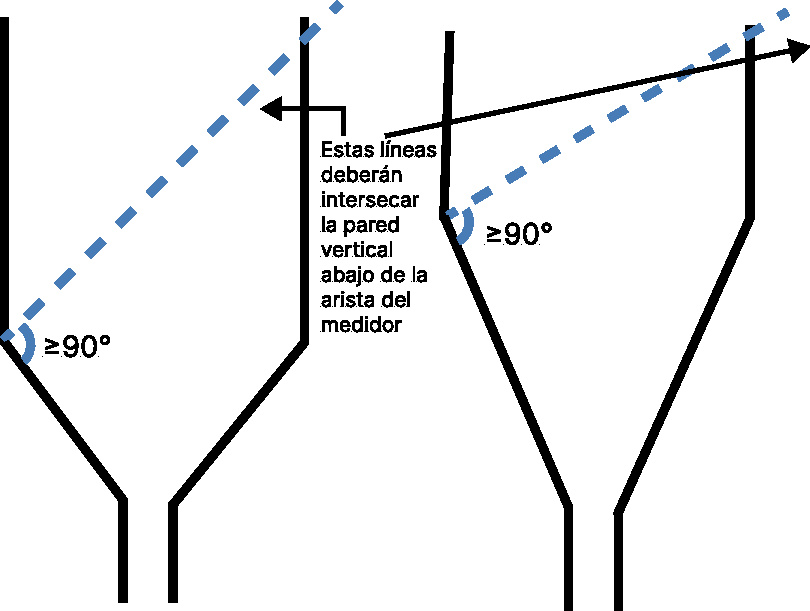
\includegraphics[width=0.5\textwidth]{t1.pdf}
  \caption{Colectaros adecuados para los pluviómetros según la norma NMX-AA-166/1-SCFI-2013 (\cite{se2013})}
  \label{t1}
\end{figure}



















\newpage
\section{Acceso a datos meteorológicos de zonas de montaña en México}
% TODO

Actualmente, no existen estaciones meteorológicas instaladas en los montes (TODO: Buscar cita), sin embargo se encontraron estaciones como en el caso del valle de México, la cuál está ubicada en el Izta-Popo y es propiedad de la UNAM

Así mismo, se pueden encontrar radares meteorológicas como es el caso de las cruces. 

Esto indica que es muy escaza la información

















\newpage
\section{Revisión de estudios previos sobre monitoreo ciudadano meteorológico}

Un artículo publicado en RMetS por Samuel Michael Illingworth et al., titulado “Red de ciudadanos sobre precipitaciones del Reino Unido: un estudio piloto”, describe cómo se utilizó GoogleChart para llevar un registro colaborativo de las precipitaciones.(\cite{illingworth2021ukprecipitation}) 

Por otro lado, el artículo “Enhancing Engagement of Citizen Scientists to Monitor Precipitation Phase” menciona la aplicación Mountain Rain or Snow, una colaboración financiada por la NASA entre Lynker, Desert Research Institute y la Universidad de Nevada-Reno. Esta aplicación permite a los usuarios reportar si está lloviendo o nevando en un momento y lugar determinados.(\cite{lute2021enhancing})


En el contexto de África, el artículo “Evaluation of Factors Affecting the Quality of Citizen Science Rainfall Data in Akaki Catchment, Addis Ababa, Ethiopia” aborda los factores que influyen en la calidad de los datos sobre precipitaciones recolectados por científicos ciudadanos.(\cite{tedla2022evaluation}) 

Asimismo, la aplicación iFlood, mencionada en el estudio “Coastal Flooding Generated by Ocean Wave- and Surge-Driven Groundwater Fluctuations on a Sandy Barrier Island”, tiene un enfoque similar, pero está diseñada específicamente para reportar inundaciones.(\cite{elgar2021coastal}) 


Otras iniciativas destacan el uso de la ciencia ciudadana para monitorear la calidad del agua y llenar vacíos de datos para cumplir con los Objetivos de Desarrollo Sostenible de las Naciones Unidas, como se describe en el artículo “Using Citizen Science to Understand River Water Quality While Filling Data Gaps to Meet United Nations Sustainable Development Goal 6 Objectives”.(\cite{mcginn2021using})

En un enfoque relacionado, el desarrollo de aplicaciones móviles para el monitoreo de aguas subterráneas también ha sido promovido como una herramienta para involucrar a la ciencia ciudadana, según se menciona en el estudio “Groundwater Mobile App Development to Engage Citizen Science”.(\cite{dennis2019groundwater})



véase la figura 2 para ubicar sus categorías.















\newpage
\section{Tecnologías actuales en monitoreo climático}
La implementación de herramientas tecnológicas para el monitoreo de fenómenos climáticos ha demostrado ser una estrategia eficiente, especialmente cuando se combina con enfoques de ciencia ciudadana. Este estudio, al fomentar la colaboración comunitaria y el uso de tecnologías accesibles, tiene el potencial de generar información crítica para el manejo de los ecosistemas de montaña.



\subsection{Pluviómetros con IoT}

\subsection{Estaciones meteorológicas}

Datos satelitales y radar metereológico: No existe la validación ni calibración. Hay información satelital que tiene dos cosas: El tamaño de pixel es muy grande y lo que está estimando() no midiendo, no se sabe qué tanto coincide con lo que hay en superficie lo real porque no hay datos, nosotros estamos generando estos datos.

En un futuro estos sirva para mejorar las estimaciones satelitales

Poner artículo donde pusieron en Canoas Altas, pero lo abandonaron, y no hay pase pública que hayan compartido


\subsection{Aplicaciones móviles}

Entre los avances más destacados está el proyecto Cooperative Open Online Landslide Repository (COOLR), que utiliza las aplicaciones \textbf{Landslide Reporter} y \textbf{Landslide Viewer}. Estas herramientas invitan a científicos ciudadanos de todo el mundo a contribuir con reportes de eventos de deslizamientos de tierra, mejorando la investigación y predicción de desastres.\cite{coolr2021} 

Además, la aplicación \textbf{Sense-it} ofrece un kit de herramientas de sensores para la investigación ciudadana, funcionando como una herramienta educativa en dispositivos Android.\cite{van2017senseit}


Otra categoría importante son los diarios de lluvia, como la aplicación \textbf{Rain Tracker} de Callum Hill, que permite a los usuarios gestionar sus propios datos de precipitaciones, aunque estos no son accesibles al público. \cite{hill2021raintracker}

Aplicaciones similares encontradas en el mercado de aplicaciones a junio de 2025, como \textbf{Pocket Rain Gauge}, \textbf{Rainlogger} y \textbf{Rain Recorder} registran las precipitaciones en función de la ubicación mediante GPS, pero tampoco ofrecen un sistema de registro público de los datos.


\subsection{Importancia hidrológica de las zonas de montaña}











\newpage
\section{Aportes del monitoreo ciudadano a la ciencia climática}



Aporta información para comprender diferentes aspectos: conocer la influencia que tiene la lluvia en los bosques, cultivos y ganado, para prevenir problemas de inundaciones y sequías, y para entender el efecto de procesos como el cambio de uso de suelo sobre el agua disponible. Todo esto es muy importante para los ecosistemas naturales y para las comunidades humanas.














% \section{Programación en Flutter}




\chapter{MATERIALES Y MÉTODOS}
%  metodología estadística usada para probar las hipótesis

% diseño experimental, modelo estadístico y procedimiento de análisis


% IR ORDENANDO LOS MÉTODOS EN FUNCIÓN DE LOS OBJETIVOS. SIEMPRE LOS MÉTODOS SUELEN INICIAR CON LA DESCRIPCIÓN DEL SITIO O POBLACIÓN DE ESTUDIO. EL SITIO DE ESTUDIO ES EL MONTE TLÁLOC Y LA POBLACIÓN DE ESTUDIO SON  LAS PERSONAS QUÉ PARTICIPAN EN EL MONITOREO.

% MÉTODOS PARA CUBRIR TODOS LOS OBJETIVOS
% VER SI LA ENCUESTA ENTRA CÓMO OBJETIVO ADICIONAL O DENTRO DE EVALUACIÓN DEL NIVEL TEC.

\section{Materiales}
\subsection{Instrumentación y equipos}
\begin{itemize}
    \item Pluviómetros calibrados con botellas graduadas hechas de PET, instaladas en bases de metal cemento y madera ubicadas en los sitios de monitoreo.
    \item Dispositivos móviles con cualquier tipo de sistema operativo, para realizar pruebas de la aplicación Tláloc App .
\end{itemize}

\subsection{Infraestructura tecnológica virtual}

\begin{itemize}
        \item \textbf{Instalaciones:} Se requiere descargar los siguientes programas en sus versiones actuales: \begin{enumerate}
        \item \textbf{Kit de Desarrollo de Software}: Flutter
        \item \textbf{Entorno de Desarrollo Integrado}: Visual Studio Code y Android Studio
        \item \textbf{Herramientas de desarrollo}: Git y Visual Studio 2022  
    \end{enumerate}
    \item \textbf{Almacenamiento del código:} Se usarán los servicios de GitHub. Esta plataforma utiliza Git para proporcionar control de versiones distribuido y, a su vez, GitHub proporciona control de acceso, seguimiento de errores, solicitudes de funciones de software, gestión de tareas, integración continua a través del programa Visual Studio Code.
    \item \textbf{Servicio de Base de datos:} Se creará un proyecto en Firebase para el Hosting en la web.
    \item \textbf{Google Play Console:} Se usará para publicar el archivo .bundle a Google Play Store, para su accesibilidad de descarga en los dispositivos Android.
\end{itemize}

\section{Método}
La presente sección describe los pasos empleados, para abordar el problema central del proyecto, el cual se profundiza en el diseño y desarrollo de un algoritmo capaz de calcular valores de precipitación reales a partir de registros acumulados. Para ello, se parte de una lista de datos de entrada proporcionada por los usuarios, y se genera como salida una lista de valores corregidos que representan las mediciones reales, obtenidas mediante la resta entre cada nuevo dato y el inmediatamente anterior.

Este proceso requiere, como paso previo, el diseño de un protocolo de monitoreo participativo que motive e instruya a los usuarios en el envío constante y preciso de datos. Posteriormente, se detalla el desarrollo del algoritmo dentro del entorno de la aplicación móvil, seguido de un análisis del estado actual del proyecto con base en el nivel de maduración tecnológica.

\begin{enumerate}
  \item Protocolo de monitoreo participativo
  \item Desarrollo de la aplicación móvil
  \item Análisis del estado actual del proyecto
\end{enumerate}






\begin{figure}[h!]
    \centering
    \begin{tikzpicture}[node distance=0.8cm]
    \node (p0) [draw=orange!50, rounded corners, minimum width=8cm, minimum height=0.7cm, dashed] {Inicio};
    \node (p1) [orangebox, below=of p0] {\textbf{1. Proceso participativo con ejidatarios}};
    \node (p2) [orangebox, below=of p1] {Presentación del proyecto a las autoridades ejidales};
    \node (p3) [orangebox, below=of p2] {Talleres participativos para la identificación de \textbf{actores} y \textbf{sitios} de monitoreo};
    
    \node (p4) [yellowbox, below=of p3] {\textbf{2. Diseño técnico de monitoreo}};
    \node (p5) [yellowbox, below=of p4] {Recorridos para la caracterización de los parajes};
    \node (p6) [yellowbox, below=of p5] {Elaboración de pluviómetros y programación de la app móvil};
    \node (p7) [yellowbox, below=of p6] {Instalación de pluviómetros};
    
    \node (p8) [cyanbox, below=of p7] {\textbf{3. Campaña de difusión con público en general}};
    \node (p9) [cyanbox, below=of p8] {Campañas de mediciones};
    \node (p10) [cyanbox, below=of p9] {Publicación de resultados y premiación};
    \node (p11) [draw=cyan!50, rounded corners, minimum width=8cm, minimum height=0.7cm, dashed, below=of p10] {Final};
    
    \foreach \i/\j in {p0/p1, p1/p2, p2/p3, p3/p4, p4/p5, p5/p6, p6/p7, p7/p8, p8/p9, p9/p10, p10/p11}
      \draw [arrow] (\i) -- (\j);
    \end{tikzpicture}
    \caption{Diagrama de flujo del Protocolo de monitoreo participativo. Autoría Propia, 2025.}
      \label{t2}
\end{figure}

\subsection{Protocolo de monitoreo participativo:}

El protocolo consiste en llevar a cabo un monitoreo de lluvia que involucró tres principales etapas las cuales son: 
\begin{enumerate}
  \item Proceso participativo de ejidatarios
  \item Diseño técnico de monitoreo
  \item Campaña de difusión con público en general
\end{enumerate}
Las cuales están desglosadas en la figura \ref{t2}


\subsubsection{1. Procesos Participativos con Ejidatarios} 
El primer paso consiste en establecer contacto con los miembros de la Unión Ejidal del Monte (UEM) para presentarles el proyecto y generar alianzas para su desarrollo. Posteriormente llevar a cabo talleres participativos con cada grupo ejidal (Nativitas, San Pablo Ixayoc, San Dieguito, Tequexquinahuac, Santa Catarina del Monte) para identificar a las personas que potencialmente podrían participar en el monitoreo y los lugares para instalar sitios de monitoreo. Este paso se resume en estas dos actividades:
\begin{itemize}
  \item Contexto Geográfico
  \item Descripción de la población de estudio
\end{itemize}


\subsubsection*{Contexto Geográfico}
La determinación del \textbf{criterio de selección de sitios de monitoreo}, se hará después de visitar los lugares propuestos por las autoridades, se debe registrar los datos de coordenadas, altitud, pendiente, tipo de vegetación, superficie desprovista de árboles y tamaño de los árboles circundantes. 

Esta información permite identificar los sitios más adecuados para instalar los sitios de monitoreo, siguiendo las recomendaciones de la Organización Meteorológica Mundial (OMM, 2014). 

En una etapa posterior se realiza un proceso de capacitación con los Ejidatarios y público en general para el monitoreo de la lluvia. Asimismo, crear un protocolo para facilitar a los Ejidatarios el uso de la información generada en sus actividades de manejo de los bosques.

\subsubsection*{Descripción de la población de estudio}

Encuestar a la población que sube a la montaña en los sitios de monitoreo los parámetros descritos en la tabla \ref{tabt3}
\begin{table}[h!]
\centering
\begin{tabular}{@{}cc@{}}
\toprule
Tipo de parámetro & Detalle                                           \\ \midrule
Sociodemográfico      & Edad, género, nivel educativo, lugar de origen/localidad          \\
Tecnológico       & Uso de celular, internet, manejo de apps          \\
Actitudinal       & Disponibilidad, disposición a participar, interés \\
Territorial/ecológico & Conocimiento del bosque, frecuencia de visita, actividades      \\
Institucional/laboral & Tipo de relación con la zona (trabajo, recreación, supervisión) \\ \bottomrule
\end{tabular}
\caption{parámetros a identificar de la población}
\label{tabt3}
\end{table}
\newpage
\subsubsection{2. Diseño Técnico de Monitoreo}

\begin{enumerate}
    \item Construcción de los pluviómetros: con botellas de PET, y siguiendo los lineamientos de la Norma Mexicana NMX-AA-166/1-SCFI-2013 (\cite{se2013}) o de la Organización Meteorológica Mundial. La máxima capacidad de almacenamiento es de 153 mm y la escala tiene resolución de un milímetro, excepto por los primeros 5 mm que tienen resolución de 0.25 mm. Los pluviómetros se colocaron sobre bases de madera a un metro sobre el nivel del suelo cavando un hoyo de 50 centímetros de profundidad. Para evitar pérdidas de agua por evaporación se utilizan 5 mm de aceite comestible vegetal por pluviómetro, (Figura \ref{m21}).

    \item Los pluviómetros se vacían y registran por el equipo técnico con una frecuencia de un mes (más menos dos días), a menos que sea necesario vaciar con mayor frecuencia. Los participantes envían sus registros sin una frecuencia específica, por lo que sus observaciones son adicionales a las que realiza el equipo técnico. Cada estación de monitoreo cuenta con letreros que poseen la información necesaria para que las personas puedan participar aunque no se les haya dado una capacitación personal. Se cuenta con siete estaciones de monitoreo en un gradiente altitudinal que va de 2683 a 3870 m. 
\end{enumerate}


\begin{figure}[h!]
\centering
  \includegraphics[width=1\textwidth]{m21.png}
  \caption{Diseño de pluviómetro de pet}
  \label{m21}
\end{figure}






\newpage
\subsubsection{3. Campaña de difusión con público en general}

Este último paso, consiste en crear una campaña permanente de difusión entre la gente que sube a la montaña. Implica generar material gráfico instalado en campo que invite a la población a participar, trípticos y carteles que se colocan en lugares estratégicos;  utilizar las redes sociales para dar a conocer el proyecto y mecanismos para premiar a los participantes activos con regalos. 


Se plantea utilizar diversos medios y plataformas de divulgación enfocados en cada audiencia objetivo, que incluye lonas impresas, carteles, trípticos, Facebook, correos institucional y pláticas informativas. En el cuadro \ref{tab1} se muestra la descripción de medios y plataformas.

\begin{table}[h!]
    \centering
    \resizebox{\columnwidth}{!}{%
    \begin{tabular}{@{}cccc@{}}
    \toprule
    Medios y plataformas &
      Objetivo &
      Distribución &
      Audiencia objetivo \\ \midrule
    Lonas impresas &
      \begin{tabular}[c]{@{}c@{}}Difundir información\\ en sitios estratégicos\\ para incentivar la\\ participación y dar a\\ conocer el procedimiento\\ de participación.\end{tabular} &
      \begin{tabular}[c]{@{}c@{}}Se van a colocar en la\\ entrada principal a la\\ montaña (pluma de\\ acceso ubicada en el\\ sitio conocido como el\\ venturero), así como en\\ las 6 oficinas ejidales de\\ los Ejidos de la Montaña.\end{tabular} &
      Todas las audiencias \\
    Carteles &
      \begin{tabular}[c]{@{}c@{}}Dar a conocer el\\ procedimiento para\\ realizar las\\ mediciones en cada\\ sitio de monitoreo\\ de la lluvia.\end{tabular} &
      \begin{tabular}[c]{@{}c@{}}Se van a colocar en cada\\ sitio de monitoreo.\end{tabular} &
      Todas las audiencias \\
    Trípticos &
      \begin{tabular}[c]{@{}c@{}}Dar a conocer el\\ proyecto y el procedimiento de\\ participación a las\\ personas que\\ ingresan a la\\ montaña.\end{tabular} &
      \begin{tabular}[c]{@{}c@{}}Se van a repartir en la\\ entrada principal a la\\ montaña.\end{tabular} &
      \begin{tabular}[c]{@{}c@{}}Visitantes externos\\ Visitantes internos\\ Miembros de\\ instituciones gubernamentales y\\ técnicos forestales\\ Miembros de la academia\end{tabular} \\
    Página de Facebook &
      \begin{tabular}[c]{@{}c@{}}Difundir de manera\\ masiva el proyecto.\end{tabular} &
      Red social Facebook &
      Todas las audiencias \\
    Correo institucional &
      \begin{tabular}[c]{@{}c@{}}Difundir el proyecto\\ en la comunidad\\ COLPOS.\end{tabular} &
      Correo Colpos &
      Miembros de la academia \\
    Pláticas informativas &
      \begin{tabular}[c]{@{}c@{}}Dar a conocer e\\  proyecto y el\\ procedimiento de\\ participación con\\ determinadas\\ audiencias objetivo.\end{tabular} &
      \begin{tabular}[c]{@{}c@{}}Se realizó en etapas\\ previas de preparación\\ del proyecto con cada\\ Comité Ejidal. También\\ se va a llevar a cabo una\\ reunión con académicos\\ que realizan trabajo en\\ el Monte Tláloc.\end{tabular} &
      \begin{tabular}[c]{@{}c@{}}Ejidatarios de la Unión\\ de Ejidos de la Montaña\\ y sus cuadrillas de trabajo\\ Miembros de la academia\end{tabular} \\ \bottomrule
    \end{tabular}%
    }
    \caption{Medios y plataformas de divulgación del proyecto ``Ciencia ciudadana para el monitoreo participativo de la lluvia en un gradiente altitudinal del Monte Tláloc, Texcoco, estado de México''}
    \label{tab1}
    \end{table}


\subsubsection*{Descripción de información para los medios y plataformas de divulgación}

\begin{enumerate}
    \item \textbf{Lonas impresas:}
    \begin{enumerate}
        \item Título del proyecto:
        Proyecto ``Ciencia ciudadana para el monitoreo de la lluvia en un gradiente altitudinal del Monte Tláloc, Texcoco, estado de México”
        \item	Slogan: 
        ``Ciencia para ti y para todos''
        \item Logo del proyecto
        \item Logo del COLPOS y Postgrado en Ciencias Forestales
        \item Frase: Unión de Ejidos de la Montaña (junto a los logos del COLPOS y PCF)
        \item Texto principal: ¡Te invitamos a colaborar en el monitoreo de la lluvia en el Monte Tláloc, es muy sencillo!
        \item Diagrama de flujo con imágenes: \begin{enumerate}
            \item Ubica un sitio de monitoreo.
            \item Observa cuánta lluvia está almacenada en el pluviómetro.
            \item Envíanos la información (nivel del agua, fecha y hora del día) y una fotografía, con la aplicación móvil Tláloc app o por WhatsApp.
            \item Croquis del monitoreo
            \item Información complementaria: Cada 30 días se premiará con un obsequio muy especial a los 3 participantes con más registros. Además, al            registrarte en Tláloc App podrás tener acceso a la información que            generemos entre todos. Descarga Tláloc App en (poner sitio de descarga). Consulta más información en (poner la página de Facebook) o mándanos un WhatsApp para asesorarte (poner número telefónico). ¡Ayúdanos a mantener en condiciones adecuadas los instrumentos de
            medición!
        \end{enumerate}
    \end{enumerate}
    \item \textbf{Cartel frontal} \begin{enumerate}
        \item Slogan: 
        Ciencia para ti y para todos (quizás rodeando el logo del proyecto, en letra pequeña)
        \item Logo del proyecto (que destaque más que los otros logos)
        \item Logo del COLPOS y Postgrado en Ciencias Forestales
        \item Frase: Unión de Ejidos de la Montaña (junto a los logos del COLPOS y PCF)
        \item Texto principal: ¡Te invitamos a colaborar en el monitoreo de la lluvia en el Monte Tláloc!
        \item Tutorial \begin{enumerate}
            \item Observa el pluviómetro agachándote hasta que el nivel del agua esté frente a tus ojos. 
            \item Ubica la línea más cercana al nivel del agua y registra tu medición. 
            Poner esquema de cómo observar y una ampliación a cómo se ve el nivel de agua y la escala de medición.
            \item Registra tu medición con Tláloc App:
            
            Abre la aplicación e inicia sesión (colaborador externo o monitor); Escanea el código QR ubicado en la base del Pluviómetro; Registra tu medición en el espacio “Precipitación en mm”; Verifica que la fecha  y hora de la aplicación son correctas o edítalas si es necesario (poner los íconos de fecha y hora);Toma una foto del pluviómetro en la que se vea el nivel del agua como una línea. (poner una foto correcta y una incorrecta)            
            \item 	Si no cuentas con Tláloc App, anota los siguientes datos y mándalos con Whats App: Clave del pluviómetro ubicada en la base del Pluviómetro; Resultado de tu medición (Precipitación en mm); Fecha y hora; Foto del pluviómetro en la que se vea el nivel del agua como una línea. (ver las indicaciones arriba); Nunca vacíes el pluviómetro, sólo personal autorizado puede hacerlo. ¡Muchas gracias por tu contribución!            
        \end{enumerate}
    \end{enumerate}
    \item \textbf{Cartel posterior} \begin{enumerate}
        \item Título del proyecto: Proyecto “Ciencia ciudadana para el monitoreo de la lluvia en un gradiente altitudinal del Monte Tláloc, Texcoco, estado de México”
        \item Logo del COLPOS y Postgrado en Ciencias Forestales
        \item Frase: Unión de Ejidos de la Montaña
        \item Texto principal: Este es un pluviómetro. Tiene una escala de medición en milímetros que indica la cantidad de lluvia que cae por metro cuadrado de terreno.
        \item Esquema del pluviómetro y la equivalencia de un mm de lluvia (1 mm = a vaciar un litro de agua en cada metro cuadrado de terreno).
        \item Saber cuándo, dónde y cuánto llueve en la montaña ayuda a entender cómo conservar el bosque y el agua que viene de ella. Cada 30 días se premiará a los 3 participantes con más registros. Además, al registrarte en Tláloc App podrás tener acceso a la información que generemos entre todos. Descarga Tláloc App en (poner sitio de descarga). Consultar más información en Facebook o mándanos un WhatsApp para asesorarte. ¡Ayúdanos a cuidar este pluviómetro! Por favor reporta si encuentras dañado este sitio de monitoreo.
    \end{enumerate}
    % \item \textbf{Tríptico}
    % \item \textbf{Página de Facebook}
    % \item \textbf{Pláticas informativas}
\end{enumerate}





































































\subsection{Desarrollo del código}
En este sistema de monitoreo participan tres elementos principales: el usuario, el pluviómetro y la aplicación multiplataforma. El usuario es la persona encargada de registrar las mediciones realizadas por el pluviómetro artesanal, instalado en un paraje específico. Esta interacción ocurre a través de un código QR asignado a cada pluviómetro, el cual permite vincularlo con su ubicación y sus datos de monitoreo.

La aplicación multiplataforma facilita esta interacción al estar disponible en diferentes dispositivos como teléfonos inteligentes, tabletas, laptops o computadoras de escritorio, y puede ejecutarse en sistemas operativos como Android, iOS, Huawei OS, Windows y navegadores web. De este modo, el usuario puede elegir el dispositivo de su preferencia para capturar y enviar los datos registrados por el pluviómetro al sistema.

La Figura \ref{t3}, muestra el diagrama de flujo que representa el comportamiento operativo del sistema y cómo se realiza el intercambio de información entre estos tres actores.
\begin{figure}[h!]
\centering
  \includegraphics[width=1\textwidth]{t3.pdf}
  \caption{Diagrama de flujo de trabajo del sistema de Pluviómetros con Tláloc App}
  \label{t3}
\end{figure}

La metodología para el desarrollo del código, consiste en programar en lenguaje Dart, una aplicación multiplataforma, alojada en un sitio web y en Play Store, con el fin de enviar las mediciones a una base de datos pública bajo la siguiente organización:


\begin{enumerate}
  \item \textbf{Backend}
  \begin{enumerate}
    \item Alojamiento del código: Exportar y guardar en GitHub
    \item Base de datos: Lógica del código, seguridad y conexión en Firebase
    \item Hosting en la web: Publicar un dominio en Firebase
  \end{enumerate}
  \item \textbf{Frontend}
  \begin{enumerate}
    \item User Experience (UX)
     \begin{enumerate}
      \item Material Design
      \item Acceso en tienda de aplicaciones (PlayStore)
     \end{enumerate}
    \item User Interface (UI)
    % : se construye a partir de widgets, que son unidades reutilizables de interfaz. Estos widgets permiten definir pantallas de forma declarativa, promoviendo una organización jerárquica clara y facilitando el mantenimiento del código. Un diseño de UI eficiente no solo debe ser estéticamente agradable, sino también funcional, accesible y coherente con los principios de diseño establecidos (como Material Design). Las pantallas a mostrar son las siguientes:
    \begin{enumerate}
    \item Onboarding: Pagina de bienvenida 
    \item Login: Los usuarios podrán crear una cuenta y elegir el pluviómetro mediante el escaneo de códigos Qr o manualmente del sitio de monitoreo 
    \item Menú Principal: Dispondrá de tutoriales, contador de mediciones, acerca de, tabulador de mediciones, mapas de las dos rutas, grupos para subir a la montaña y contacto
    \item Envío de mediciones: Incluye campo de texto, pluviómetro interactivo, booleano de vaciado, cambio de paraje
    \item Bitácora: Disponibilidad de consulta, edición, difusión o eliminación de las mediciones propias y no de otros usuarios; y exportación en excel.
    \item Estadísticas: Mostrará un gráfico interactivo en diferentes tiempo de interés, por ejemplo por semana, mes y año; entre volúmenes acumulados y reales.
\end{enumerate}
  \end{enumerate}
\end{enumerate}











\newpage
\subsubsection{1a. Configuración en GitHub}

\subsubsection*{Control de versiones y almacenamiento en GitHub}

El desarrollo de aplicaciones requiere no solo un diseño estructurado del código, sino también un control riguroso de versiones y respaldos. GitHub es una plataforma ampliamente usada en el ámbito académico y profesional para alojar proyectos de software, permitiendo la colaboración, el seguimiento de cambios y el resguardo del historial del código fuente. 

Para este proyecto, el repositorio deberá publicarse en GitHub:
\begin{center}
\url{https://github.com}
\end{center}

\subsubsection*{Proceso para guardar código localmente en GitHub con Git}

El flujo básico para controlar versiones de un proyecto usando \texttt{git} desde la computadora incluye los siguientes pasos:

\begin{enumerate}
    \item Inicializar el repositorio en la carpeta del proyecto (solo la primera vez):
    \begin{minted}{bash}
    git init
    \end{minted}
    
    \item Configurar nombre y correo del autor (también solo una vez):
    \begin{minted}{bash}
    git config --global user.name "Luis Emilio Álvarez Herrera"
    git config --global user.email "ejemplo@dominio.com"
    \end{minted}
    
    \item Agregar el repositorio remoto de GitHub:
    \begin{minted}{bash}
    git remote add origin https://github.com/Jack55913/TlalocApp.git
    \end{minted}
    
    \item Verificar el estado del repositorio y los archivos modificados:
    \begin{minted}{bash}
    git status
    \end{minted}
    
    \item Añadir los archivos que se desean guardar (todos o algunos específicos):
    \begin{minted}{bash}
    git add .
    \end{minted}
    
    \item Registrar los cambios con un mensaje claro:
    \begin{minted}{bash}
    git commit -m "Primera versión de Tláloc App"
    \end{minted}
    
    \item Subir los cambios al repositorio remoto en GitHub:
    \begin{minted}{bash}
    git push -u origin main
    \end{minted}
\end{enumerate}

Este flujo se puede repetir cada vez que se realicen avances importantes en el código. Gracias a Git, cada modificación queda registrada con fecha, autor y propósito, lo cual facilita el mantenimiento del software, el trabajo colaborativo y la trazabilidad científica del desarrollo.

\subsubsection*{Clonar el repositorio desde GitHub}

Si se necesita obtener una copia exacta del proyecto alojado en GitHub en otra computadora, es posible usar el comando \texttt{git clone}. Este comando descarga todo el historial y los archivos del proyecto:

\begin{minted}{bash}
git clone https://github.com/Jack55913/TlalocApp.git
\end{minted}

Este comando crea automáticamente una carpeta llamada \texttt{TlalocApp} con todos los archivos y el historial del proyecto.

\subsubsection*{Subir cambios al repositorio remoto: \texttt{git push}}

Una vez realizados cambios en el código, es posible subirlos a GitHub con el siguiente flujo:

\begin{enumerate}
    \item Verificar el estado del repositorio local:
    \begin{minted}{bash}
    git status
    \end{minted}
    
    \item Agregar los archivos modificados al área de preparación:
    \begin{minted}{bash}
    git add .
    \end{minted}
    
    \item Registrar los cambios localmente con un mensaje:
    \begin{minted}{bash}
    git commit -m "Descripción clara del cambio realizado"
    \end{minted}
    
    \item Subir los cambios al servidor de GitHub:
    \begin{minted}{bash}
    git push origin main
    \end{minted}
\end{enumerate}

Este proceso permite mantener actualizado el repositorio en la nube, sirviendo como respaldo y facilitando el trabajo colaborativo.

\subsubsection*{Obtener actualizaciones del repositorio remoto: \texttt{git pull}}

Si se ha trabajado en el mismo repositorio desde otra computadora o por otros colaboradores, se deben sincronizar los cambios con:

\begin{minted}{bash}
git pull origin main
\end{minted}

Este comando fusiona los cambios realizados en GitHub con la copia local del proyecto. Es recomendable ejecutarlo antes de comenzar una nueva sesión de desarrollo para evitar conflictos.


















\subsubsection{1b. Configuración en Firebase} 
Para establecer una conexión efectiva entre una aplicación desarrollada en \textit{Flutter} y el servicio de base de datos en tiempo real \textit{Firestore}, proporcionado por \textit{Firebase}, es necesario llevar a cabo una serie de configuraciones tanto en la plataforma web de Firebase como dentro del propio entorno del proyecto Flutter.

El primer paso consiste en acceder al panel de control oficial de Firebase, disponible en:

\begin{center}
  \url{https://console.firebase.google.com/}
\end{center}

Desde esta consola, se debe crear un nuevo proyecto seleccionando la opción \texttt{Agregar proyecto}, asignándole un nombre distintivo y, de forma opcional, desactivando Google Analytics según los requerimientos de privacidad. Una vez creado el proyecto, se procede a registrar las plataformas de destino, por ejemplo, \textit{Android} y \textit{Web}, haciendo clic en los íconos correspondientes.

\vspace{1em}

\paragraph{Configuración en Android.}  
Para Android, se solicita un identificador de paquete único, en este caso:

\begin{center}
  \texttt{com.TlalocApps.tlaloc}
\end{center}

Este identificador debe coincidir exactamente con el declarado en el archivo \texttt{android/app/build.gradle}. Al registrar la app, Firebase generará un archivo de configuración llamado \texttt{google-services.json}, el cual debe descargarse y colocarse dentro del directorio \texttt{android/app/} del proyecto Flutter.

\vspace{1em}

\paragraph{Configuración en Web.}  
En el caso de aplicaciones web, se debe registrar un nombre de dominio o ID de aplicación. Al finalizar, Firebase genera un bloque de código JavaScript con claves como \texttt{apiKey}, \texttt{projectId} y \texttt{messagingSenderId}. En Flutter, basta con integrar estas claves a través de un archivo generado automáticamente, como se explica más adelante.

\vspace{1em}

\paragraph{Instalación de dependencias.}  
Dentro del archivo \texttt{pubspec.yaml}, se deben agregar los paquetes necesarios para la conexión con Firebase, en este caso:

\begin{center}
  \texttt{firebase\_core}, \quad
  \texttt{cloud\_firestore}, \quad
  \texttt{firebase\_auth}, \quad
  \texttt{firebase\_storage}
\end{center}

Posteriormente, se deben instalar con el comando:

\begin{center}
  \texttt{flutter pub get}
\end{center}

\vspace{1em}

\paragraph{Inicialización de Firebase.}  
En el archivo principal \texttt{main.dart}, es indispensable inicializar Firebase antes de correr la aplicación, utilizando:

\begin{center}
  \texttt{await Firebase.initializeApp();}
\end{center}

Esto se hace dentro de la función \texttt{main()} para evitar errores de ejecución asíncrona, usando:
\begin{center}
  \texttt{WidgetsFlutterBinding.ensureInitialized()}
\end{center}

\vspace{1em}

\paragraph{Ajustes específicos en Android.}  
Se requiere modificar el archivo \texttt{android/build.gradle} para añadir el siguiente classpath dentro de la sección \texttt{dependencies}:

\begin{center}
  \texttt{classpath 'com.google.gms:google-services:4.3.15'}
\end{center}

Asimismo, en \texttt{android/app/build.gradle} se debe aplicar el plugin:

\begin{center}
  \texttt{apply plugin: 'com.google.gms.google-services'}
\end{center}

También es recomendable asegurar que la versión mínima de SDK sea \texttt{minSdkVersion 23} o superior, y que las versiones de \texttt{Kotlin} y \texttt{Gradle} sean compatibles con Firebase.

\vspace{1em}

\paragraph{Configuración multiplataforma con FlutterFire CLI.}  
Para simplificar la configuración de Firebase en todas las plataformas, se recomienda utilizar la herramienta oficial de línea de comandos para Flutter, mediante el siguiente comando:

\begin{center}
  \texttt{flutterfire configure}
\end{center}

Este comando genera automáticamente el archivo \texttt{firebase\_options.dart}, el cual contiene la configuración centralizada para \texttt{Android}, \texttt{iOS}, \texttt{macOS} y \texttt{Web}. En el código, se debe inicializar Firebase con:

\begin{center}
  \texttt{Firebase.initializeApp(options: DefaultFirebaseOptions.currentPlatform);}
\end{center}

Esto garantiza una inicialización adecuada en cualquier dispositivo desde el que se ejecute la aplicación.

\vspace{1em}

Con esta configuración correctamente establecida, la aplicación Flutter puede acceder de forma segura y eficiente a Firestore, lo cual permite implementar funcionalidades como autenticación, almacenamiento, y sincronización de datos en tiempo real entre usuarios y dispositivos.


\subsubsection{1c. Web Hosting}
Además del almacenamiento de datos, se habilitó el servicio de \textbf{Firebase Hosting} para desplegar una versión web de la aplicación. Este entorno permite servir contenido estático y dinámico mediante HTTPS, ofreciendo una plataforma confiable y segura para la visualización pública de estadísticas y reportes.

La implementación del hosting se realizó con los siguientes pasos:

\begin{enumerate}
    \item Instalación de las herramientas de línea de comandos de Firebase (\texttt{firebase-tools}).
    \item Inicialización del proyecto con \texttt{firebase init} y selección de las funciones de Hosting.
    \item Configuración del directorio de salida del proyecto web compilado con Flutter.
    \item Despliegue del sitio mediante el comando \texttt{firebase deploy}.
\end{enumerate}






\subsubsection{2a. User Experience}

Para diseñar una experiencia de usuario (UX) sólida y centrada en las necesidades reales de las personas usuarias, es fundamental comprender y aplicar la estructura (\cite{garrett2011elements}), quien descompone la experiencia del usuario en cinco planos jerárquicos e interdependientes. 

Estos planos permiten están esquematizados en la figura \ref{m7}, y abordan el diseño desde la abstracción estratégica hasta su implementación visual concreta. 

\begin{enumerate}
  \item En primer lugar, el plano de la \textbf{estrategia} define los objetivos tanto del usuario como del proyecto, estableciendo el ``por qué'' detrás del sistema. 
  
   \item A continuación, el plano del \textbf{alcance} transforma estos objetivos en requerimientos funcionales (como las características del sistema) y requerimientos de contenido (como textos, imágenes o formularios).

 \item El tercer plano corresponde a la \textbf{estructura}, que se refiere a cómo se organizan las funciones y el contenido dentro del sistema, abarcando tanto la arquitectura de la información como el diseño de la interacción. 
 
  \item Posteriormente, el plano del \textbf{esqueleto} define el diseño de la interfaz, la navegación y la disposición de los elementos para asegurar la usabilidad, que para este caso se usó el programa Figma para elaborar diseñar. 
  \begin{center}
    \url{https://www.figma.com/}
  \end{center}
  
   \item El último plano llamado \textbf{superficie}, es la capa visual con la que el usuario interactúa directamente, incluyendo la elección de colores, tipografía, iconografía y estilo gráfico. Este modelo secuencial permite una toma de decisiones coherente y una alineación efectiva entre las necesidades del usuario y los objetivos del proyecto. Para el presente proyecto se usó Material Design 3:
   \begin{center}
    \url{https://m3.material.io/}
   \end{center}
\end{enumerate}


\begin{figure}[h!]
\centering
  \includegraphics[width=0.9\textwidth]{m7.jpg}
  \caption{El modelo delineado busca definir las consideraciones clave que forman el desarrollo de la experiencia de usuario (\cite{garrett2011elements}).}
  \label{m7}
\end{figure}

\newpage
\subsubsection*{Tiendas de aplicaciones}
Para publicar una aplicación Flutter en la Google Play Store requiere seguir una serie de pasos técnicos y administrativos que garantizan la calidad, seguridad y compatibilidad del producto final. A continuación se describe el proceso completo para llevar la app desde el entorno de desarrollo hasta su disponibilidad pública en la tienda.

\paragraph{1. Crear una cuenta de desarrollador en Google Play}

Antes de iniciar el proceso técnico, se debe crear una cuenta en la Play Console (\url{https://play.google.com/console}) como desarrollador. Esto requiere:

\begin{itemize}
    \item Una cuenta de Google personal o institucional.
    \item El pago único de una tarifa de registro (25 USD al momento de la redacción).
    \item Aceptar los términos y condiciones de Google Play.
\end{itemize}

\paragraph{2. Preparar la aplicación Flutter}

Para distribuir una app Flutter en Android se deben cumplir los siguientes pasos:

\begin{enumerate}
    \item Establecer nombre del paquete de forma única en el archivo \texttt{android/app/build.gradle}, por ejemplo:
\begin{minted}{yaml}
applicationId "com.TlalocApps.tlaloc"
\end{minted}

    \item Modificar el archivo \texttt{android\/app\/src\/main\/AndroidManifest.xml} para establecer permisos, íconos y orientaciones.

    \item Establecer versión y código de versión en \texttt{pubspec.yaml}:
\begin{minted}{yaml}
version: 1.0.0+1
\end{minted}

    \item Configurar el ícono de la app usando el paquete \texttt{flutter\_launcher\_icons}:
\begin{minted}{bash}
flutter pub add flutter\_launcher_icons
flutter pub run flutter\_launcher_icons:main
\end{minted}

    \item Habilitar los modos de firma para release en \texttt{android\/key.properties} y \texttt{build.gradle}. Crear una clave de firma con:
\begin{minted}{bash}
keytool -genkey -v -keystore ~/key.jks \
  -keyalg RSA -keysize 2048 -validity 10000 \
  -alias tlaloc_key
\end{minted}

    \item Asegurar que se usa la variante \texttt{release} al compilar:
\begin{minted}{bash}
flutter build appbundle
\end{minted}

    Este comando genera un archivo \texttt{.aab} (Android App Bundle) necesario para subir la app a la Play Store.(\cite{AndroidSigning})
\end{enumerate}

\paragraph{3. Crear la ficha de Play Store}

Desde Google Play Console:

\begin{itemize}
    \item Seleccionar \textbf{Crear aplicación}.
    \item Ingresar nombre, idioma, tipo (App o Juego) y categoría (Educación, Estilo de vida, etc.).
    \item Completar la \textbf{ficha de Play Store}: título, descripción corta y larga, íconos (512x512 px), capturas de pantalla (mínimo 2), gráfico promocional opcional, política de privacidad (vínculo web).
\end{itemize}

\paragraph{4. Subir el archivo .AAB y configurar la versión}

\begin{itemize}
    \item Ir a \textbf{Release > Producción > Crear nueva versión}.
    \item Cargar el archivo \texttt{.aab} generado.
    \item Agregar notas de la versión.
    \item Establecer políticas de uso, permisos solicitados y nivel mínimo de API.
\end{itemize}

\paragraph{5. Clasificación de contenido y verificación}

Se debe:

\begin{itemize}
    \item Responder el cuestionario de clasificación por edades.
    \item Completar la sección de seguridad de datos y uso de bibliotecas externas (Firebase, Google Sign-In, etc.).
    \item En algunos casos, aceptar la revisión previa de funciones sensibles.
\end{itemize}

\paragraph{6. Publicar la aplicación}

Una vez completado todo el proceso anterior:

\begin{itemize}
    \item Se envía la aplicación para revisión.
    \item El proceso puede tardar entre 24 a 72 horas.
    \item Si es aprobada, aparecerá públicamente en la Play Store en cuestión de horas.
\end{itemize}

\paragraph{7. Actualizaciones posteriores}

Cada vez que se realiza una actualización, se debe:

\begin{enumerate}
    \item Incrementar el código de versión en \texttt{pubspec.yaml}.
    \item Generar un nuevo archivo \texttt{.aab}.
    \item Subir la nueva versión en \textbf{Play Console}.
\end{enumerate}





\subsubsection{2b. User Interface}

El desarrollo de una aplicación móvil requiere no solo la implementación funcional del código, sino también una organización arquitectónica sólida basada en principios de programación orientada a objetos (POO). Esta metodología permite estructurar el proyecto en módulos bien definidos, reutilizables y escalables, facilitando la colaboración, el mantenimiento y la evolución del software a largo plazo.

En el contexto de Flutter, un framework multiplataforma basado en el lenguaje Dart, la programación orientada a objetos se refleja en la creación de clases, componentes y funciones que encapsulan el comportamiento y la lógica de la interfaz, el manejo de datos y la interacción con servicios externos. Cada parte de la aplicación se define como un widget o clase independiente, lo que promueve una arquitectura limpia y modular.

Un proyecto de programación orientada a objetos bien estructurado debe cumplir con los siguientes principios fundamentales:

\begin{enumerate}
    \item \textbf{Encapsulamiento}: Separar la lógica interna de los objetos del acceso externo mediante funciones o métodos bien definidos.
    \item \textbf{Abstracción}: Definir estructuras lógicas que representen entidades clave del sistema (usuarios, mediciones, parajes, etc.).
    \item \textbf{Herencia}: Reutilizar comportamientos comunes a través de clases base o mixins cuando sea necesario.
    \item \textbf{Polimorfismo}: Permitir la utilización de interfaces genéricas que se comportan de forma diferente según el contexto.
\end{enumerate}



\subsection{Evaluación del nivel de maduración tecnológica}

El modelo del CONACyT, ahora SECIHTI, ha derivado la Norma Oficial Mexicana NMX-GT-004-IMNC-2012, identifica cada nivel de TRL por medio de una lista de verificación con preguntas dicotómicas con respuestas de ``si'' o ``no'', lo que permite que la herramienta sea eficiente.


El Nivel de Madurez Tecnológica (NMT o Technology Readiness Level, TRL, en inglés) 
Es una escala de medición usada para evaluar o medir el nivel de madurez de una
tecnología particular. Cada proyecto es evaluado frente a los parámetros de cada
nivel tecnológico y es asignado a una clasificación basada en el progreso del
proyecto.

Para la presente investigación, apoyándose de la figura \ref{m19}, se hará la evaluación del nivel de maduración tecnológica de Tlaloc App.

\begin{figure}[h!]
\centering
  \includegraphics[width=1\textwidth]{m19.png}
  \caption{Guía para el Diagnóstico del Nivel de Madurez Tecnológica (NMT o TRL, por sus siglas en inglés) (\cite{SECIHTIConvocatorias}).}
  \label{m19}
\end{figure}

\chapter{RESULTADOS Y DISCUSIÓN}
% comparativas con otras plataformas, aunque sean preliminares.


% tasas de participación de usuarios, número de lluvias registradas, precisión de mediciones    
\section{Protocolo de monitoreo participativo:}
  % \item Proceso participativo de ejidatarios
\subsection{Proceso participativo de ejidatarios}
\subsubsection{Descripción de los sitios de monitoreo}

El Monte Tláloc es un volcán ubicado en el Eje Neovolcánico, en el límite territorial de los municipios de Ixtapaluca y Texcoco, al oriente del estado de México. Forma parte de la Sierra Nevada y se encuentra dentro del Área Natural Protegida denominada \textit{Parque Nacional Iztaccíhuatl-Popocatépetl}. Su localización hidrológica corresponde a la región oriental de la cuenca de México.

Geológicamente, se trata de una estructura volcánica conformada por capas de sucesivas erupciones basálticas de carácter fluido. Su altitud alcanza los 4,120 metros sobre el nivel del mar, lo que lo posiciona como la novena cima más alta del país. El clima predominante es de tipo montaña, clasificado oficialmente como semifrío subhúmedo con lluvias en verano y humedad media \cite{inegi_texcoco}.

Los sitios de monitoreo seleccionados para esta investigación fueron definidos conforme a los criterios establecidos en la metodología, tales como coordenadas, altitud, pendiente, tipo de vegetación, superficie desprovista de árboles y tamaño de los árboles circundantes. La validación de dichos sitios se documenta en la Tabla~\ref{tabrsm1}, correspondiente a la bitácora de campo. Además, el proceso de selección queda evidenciado a través de las Figuras~\ref{m12} y~\ref{m13}.


\begin{figure}[ht]
\centering
  \includegraphics[width=0.5\textwidth]{m12.jpg}
  \caption{Medición de espacio entre arboles}
  \label{m12}
\end{figure}
\begin{figure}[ht]
\centering
  \includegraphics[width=0.5\textwidth]{m13.jpg}
  \caption{Medición de altura de árboles con un altímetro}
  \label{m13}
\end{figure}

% TODO: COMPLETAR DATOS
\begin{landscape}
\begin{table}[h!]
\centering
\resizebox{\columnwidth}{!}{%
\begin{tabular}{@{}ccccccccc@{}}
\toprule
Sitio /   Caract. &
  \textbf{El Venturero} &
  \textbf{El Jardín} &
  \textbf{Cabaña} &
  \textbf{Cruz de Atenco} &
  \textbf{Canoas altas} &
  \textbf{Los Manantiales} &
  \textbf{Tlaltlatlately} &
  \textbf{Agua de Chiqueros} \\ \midrule
Ejido &
  Nativitas &
  Nativitas &
  \begin{tabular}[c]{@{}c@{}}Sn Pablo\\ Ixayoc\end{tabular} &
  \begin{tabular}[c]{@{}c@{}}San\\ Dieguito\end{tabular} &
  \begin{tabular}[c]{@{}c@{}}San\\ Dieguito\end{tabular} &
  Tequexquinahuac &
  \begin{tabular}[c]{@{}c@{}}Santa Catarína\\ del Monte\end{tabular} &
  \begin{tabular}[c]{@{}c@{}}Santa Catarína\\ del Monte\end{tabular} \\
\textit{\begin{tabular}[c]{@{}c@{}}Tipo de \\  Vegetación\end{tabular}} &
  \begin{tabular}[c]{@{}c@{}}Encinos\\ y mixto\end{tabular} &
  \begin{tabular}[c]{@{}c@{}}Abies\\ religiosa\end{tabular} &
  \begin{tabular}[c]{@{}c@{}}Encino /\\ Abies religiosa\end{tabular} &
  \begin{tabular}[c]{@{}c@{}}Abies\\ religiosa\end{tabular} &
  \begin{tabular}[c]{@{}c@{}}Abies religiosa/\\ Pinus hartwegii\end{tabular} &
  \begin{tabular}[c]{@{}c@{}}Pinus\\ hartwegii\end{tabular} &
  \begin{tabular}[c]{@{}c@{}}Encinos y\\ mixto\end{tabular} &
  Pinus hartwegii \\
\multicolumn{9}{c}{\textbf{CARACTERÍSTICAS TOPOGRÁFICAS}} \\
\textit{\begin{tabular}[c]{@{}c@{}}Altitud\\      (msnm)\end{tabular}} &
  2683 &
  2977.3 &
  3064.3 &
  3435.4 &
  3515.1 &
  3625.3 &
  2980.5 &
  3727.3 \\
\textit{Latitud N} &
  19°27'44.40'' &
  19°26.6800' &
  19°25.3800' &
  19°25.0520' &
  19°23.6810' &
  19°23.6810' &
  19°27.8780' &
  19°26.3550' \\
\textit{Longitud   O} &
  98°47'28.66'' &
  98°46.3200' &
  98°45.8170' &
  98°45.4090' &
  98°45.0420' &
  98°43.6380' &
  98°45.9280' &
  98°43.1340' \\
\textit{\begin{tabular}[c]{@{}c@{}}Ancho\\ del   \\ paraje (m)\end{tabular}} &
  ? &
  35 &
  15 &
  70 &
  32 &
  125 &
  67 &
  110 \\
\textit{\begin{tabular}[c]{@{}c@{}}Largo\\ del   \\ paraje (m)\end{tabular}} &
  ? &
  45 &
  50 &
  79 &
  56 &
  189 &
  134 &
  191 \\
\begin{tabular}[c]{@{}c@{}}Condición\\ de la\\ barrera de\\ árboles\end{tabular} &
  ? &
  ? &
  ? &
  \begin{tabular}[c]{@{}c@{}}Barrera\\ completa\\ de árboles\\ de aprox\\ 20 m\end{tabular} &
  ? &
  \begin{tabular}[c]{@{}c@{}}Rodeado\\ de árboles\\ en el 75\%\\ del área,\\ hay mucho\\ viento.\end{tabular} &
  \begin{tabular}[c]{@{}c@{}}Árboles de\\ hasta 20 m,\\ cima de\\ un lomerío,\\ bordeado\\ de árboles\\ de manera\\ homogénea.\end{tabular} &
  \begin{tabular}[c]{@{}c@{}}Árboles de\\ hasta 30 m. \\ Masa forestal\\ homogénea.\\ Laderas\\ que rodean\\ todo el\\ paraje.\end{tabular} \\
Accesibilidad &
  \begin{tabular}[c]{@{}c@{}}Camino\\ accesible\end{tabular} &
  \begin{tabular}[c]{@{}c@{}}Camino\\ accesible\end{tabular} &
  \begin{tabular}[c]{@{}c@{}}Camino\\ accesible\end{tabular} &
  \begin{tabular}[c]{@{}c@{}}El camino está\\ aceptable y\\ se llega\\ en\\ camioneta\\ hasta\\ el sitio\end{tabular} &
  ? &
  \begin{tabular}[c]{@{}c@{}}El camino está\\ aceptable y\\ se llega en\\ camioneta hasta\\ el sitio,\\ pero se puede\\ poner feo\\ en lluvias\end{tabular} &
  \begin{tabular}[c]{@{}c@{}}Muy accesible,\\ a pie de\\ camino y\\ en la\\ parte baja\end{tabular} &
  \begin{tabular}[c]{@{}c@{}}La última loma\\ antes de llegar al\\ sitio donde se\\ deja la camioneta\\ es difícil de subir.\\ Se caminan 500 m\\ aprox para llegar al\\ sitio de monitoreo.\end{tabular} \\
\textit{Tipo de   monitoreo} &
  Ejidal &
  Mixto &
  Mixto &
  Mixto &
  Mixto &
  Mixto &
  Ejidal &
  Mixto \\
\multicolumn{9}{c}{Pendientes Menores al 19°} \\ \bottomrule
\end{tabular}%
}
\caption{Resultados de la selección de los sitios de monitoreo}
\label{tabrsm1}
\end{table}
\end{landscape}



\subsubsection{Descripción de la población de estudio}
\label{subsubsection_pob}

La población de estudio para este trabajo se define como toda persona que participe en el proceso del monitoreo; este se compone de los siguientes grupos identificados, con características muy contrastantes:

\begin{enumerate}
    \item \textbf{Ejidatarios de la montaña (Unión de Ejidos de la Montaña) y sus cuadrillas de trabajo}: mayoritariamente hombres de entre 20 y 70 años, con nivel de estudios muy variado que llega hasta licenciatura, pero principalmente personas con educación básica a educación media. Este grupo realiza actividades de aprovechamiento forestal, incluyendo extracción de madera, musgo, perlilla y heno; y de mantenimiento del bosque (reforestación, chaponeo, podas, control de plagas, control de incendios, tendido de cercas, construcción de obras para control de erosión, remoción de suelo, mantenimiento de caminos, etc.). Algunos son residentes de las localidades propietarias de los terrenos, mientras que otros son trabajadores contratados, principalmente de Río Frío. En general suelen tener mucho trabajo, pero están dispuestos a colaborar y son los participantes del monitoreo con los que se ha tenido un contacto más estrecho. A este grupo se le va a dar una capacitación personalizada sobre el procedimiento para tomar las lecturas de los pluviómetros y se van a tener compromisos para la periodicidad de las mediciones, por lo que no es necesario convencerlos de participar.
    \item \textbf{Visitantes externos}: son todas las personas que suben a la montaña pero que no provienen de los Ejidos de la Montaña. Principalmente adultos, con gusto por convivir en ambientes naturales y con las capacidades tecnológicas necesarias para participar (teléfono móvil, acceso a internet y facilidad para el manejo de aplicaciones). En este grupo se incluyen a personas que suben de manera frecuente y son una audiencia objetivo con mucho potencial de participación, como ciclistas, senderistas, campistas y guías de turistas de empresas privadas. Otros visitantes que suben cotidianamente, pero probablemente no estén interesados en participar, son grupos de personas con alto nivel socioeconómico que se dedican a subir en motocross, jeeps y racers, cuyo objetivo es la diversión sin considerar el bienestar de la naturaleza y el impacto que generan en la zona. Finalmente, también hay visitantes externos que suben muy esporádicamente o por ocasión única, algunos suben al evento de la montaña fantasma, otros vienen del interior de la república o simplemente no tienen la costumbre de subir continuamente. Estos tres subgrupos integran una audiencia que requiere más explicación sobre los objetivos del proyecto y de cómo pueden participar y beneficiarse.
    \item \textbf{Visitantes internos}: son personas que forman parte de las localidades de los Ejidos de la Montaña pero que no trabajan con los ejidatarios, suben a realizar actividades como colecta de hongos o caminar. Es un grupo muy heterogéneo que incluye desde niños hasta adultos mayores, con mucho conocimiento sobre la zona de estudio (caminos y rutas, parajes, uso de los recursos naturales del bosque), pero probablemente no cuentan con las capacidades tecnológicas necesarias para participar (teléfono móvil, acceso a internet y facilidad para el manejo de aplicaciones).  Este grupo integra una audiencia que también requiere mucha explicación sobre los objetivos del proyecto y de cómo pueden participar y beneficiarse.
    \item \textbf{Miembros de instituciones gubernamentales y técnicos forestales}: son profesionales encargados de supervisar las actividades de aprovechamiento y manejo forestal, de los recursos del agua y el estado del bosque. Incluye a empleados de Probosque (dependencia estatal), que supervisan constantemente los trabajos realizados en la zona y apoyan en las labores de combate de incendios. También incluye a empleados de otras entidades a nivel federal como (Comisión Nacional Forestal, Comisión Nacional de Áreas Naturales Protegidas, Secretaría de Recursos Naturales, Procuraduría Federal de Protección al Ambiente y Comisión Nacional del Agua). Es un grupo integrado por adultos de entre 30 y 50 años principalmente, con mucho conocimiento sobre la zona de estudio (caminos y rutas, parajes, uso de los recursos naturales del bosque), con las capacidades tecnológicas necesarias para participar (teléfono móvil, acceso a internet y facilidad para el manejo de aplicaciones).  Aunque algunos de ellos suben continuamente, no se sabe si van a tener la disponibilidad de participar aunque sea esporádicamente, ya que siempre tienen prisa.
    \item \textbf{Miembros de la academia}: son estudiantes, profesores e investigadores que realizan actividades de investigación de muy distinta índole en la zona. Algunos suben de manera esporádica y otros suben frecuentemente. Es un grupo integrado por adultos de entre 25 y 60 años principalmente, con mucho conocimiento sobre la zona de estudio (caminos y rutas, parajes, conocimiento sobre el bosque), con las capacidades tecnológicas necesarias para participar (teléfono móvil, acceso a internet y facilidad para el manejo de aplicaciones). Algunas de las instituciones con mayor presencia en la zona son el Colegio de Postgraduados, Universidad Autónoma Chapingo, UNAM, UAM. Aunque algunos de ellos suben continuamente, no se sabe si van a tener la disponibilidad de participar aunque sea esporádicamente, ya que siempre tienen prisa.
\end{enumerate}

\begin{figure}[h!]
\centering
  \includegraphics[width=0.9\textwidth]{m14.jpg}
  \caption{Identificación de población en la montaña: Ejidatarios de la montaña}
  \label{m14}
\end{figure}

\begin{figure}[h!]
\centering
  \includegraphics[width=0.9\textwidth]{m11.jpg}
  \caption{Identificación de población en la montaña: Visitantes externos}
  \label{m11}
\end{figure}


\newpage
\subsection{Diseño técnico de monitoreo}

% Construcción de los pluviómetros
% Imagenes del pluviómetro

\begin{enumerate}
    \item Construcción de los pluviómetros: con botellas de PET, y siguiendo los lineamientos de la Norma Mexicana NMX-AA-166/1-SCFI-2013 (\cite{se2013}) o de la Organización Meteorológica Mundial. La máxima capacidad de almacenamiento es de 153 mm y la escala tiene resolución de un milímetro, excepto por los primeros 5 mm que tienen resolución de 0.25 mm. Los pluviómetros se colocaron sobre bases de madera a un metro sobre el nivel del suelo cavando un hoyo de 50 centímetros de profundidad. Para evitar pérdidas de agua por evaporación se utilizan 5 mm de aceite comestible vegetal por pluviómetro.

    \item Los pluviómetros se vacían y registran por el equipo técnico con una frecuencia de un mes (más menos dos días), a menos que sea necesario vaciar con mayor frecuencia. Los participantes envían sus registros sin una frecuencia específica, por lo que sus observaciones son adicionales a las que realiza el equipo técnico. Cada estación de monitoreo cuenta con letreros que poseen la información necesaria para que las personas puedan participar aunque no se les haya dado una capacitación personal. Se cuenta con nueve estaciones de monitoreo en un gradiente altitudinal que va de 2683 a 3870 m. 
\end{enumerate}

En la figura \ref{publicidad2}, puede observarse la instalación de la base.

\begin{figure}[ht]
\centering
  \includegraphics[width=0.5\textwidth]{publicidad/2.jpg}
  \caption{Base para el pluviómetro}
  \label{publicidad2}
\end{figure}
\begin{figure}[ht]
\centering
  \includegraphics[width=0.3\textwidth]{publicidad/4.jpg}
  \caption{Escala de graduación para precipitación.}
		\label{publicidad4}
\end{figure}


% \begin{figure}[h!]
% 	\centering
% 	\begin{subfigure} 
% 		\centering
% 		\includegraphics[width=0.2\linewidth]{publicidad/2.jpg}
% 		\caption{Base para el pluviómetro}
% 		\label{publicidad2}
% 	\end{subfigure} 
% 	\begin{subfigure} 
% 		\centering
% 		\includegraphics[width=0.2\linewidth]{publicidad/4.jpg}
% 		\caption{Escala de graduación para precipitación.}
% 		\label{publicidad4}
% 	\end{subfigure}
% 	\caption{Resultados de la instalación de pluviómetros.}
% 	\label{publicidad24-}
% \end{figure}


La distribución resultante está marcado en el mapa de la figura \ref{m3}

\begin{figure}[h!]
\centering
  \includegraphics[width=1\textwidth]{m3.jpg}
  \caption{Rutas de monitoreo de lluvia, autoría propia}
  \label{m3}
\end{figure}




\subsection{Campaña de difusión con público en general}
Como resultado, se diseñaron y publicaron los recursos ilustrados a continuación.

\subsubsection{Carteles}

Como parte de la estrategia de difusión para fomentar la participación comunitaria en el monitoreo de lluvia en el Monte Tláloc, se elaboraron distintos materiales gráficos, incluyendo carteles informativos. Estos elementos visuales fueron diseñados para captar la atención de los pobladores locales mediante una estética colorida, lenguaje claro y conciso, así como íconos representativos de la temática pluvial. 

En la figura \ref{fig:cartel1} se muestra la versión final de uno de los carteles utilizados. Este incluye información básica sobre la aplicación, la invitación a participar en el monitoreo ciudadano y un código QR para descargar la app desde la tienda de aplicaciones.

\begin{figure}[H]
\centering
  \includegraphics[width=0.7\textwidth]{publicidad/1.jpg}
  \caption{Versión final del cartel de difusión comunitaria.}
  \label{fig:cartel1}
\end{figure}

Estos carteles fueron colocados en sitios estratégicos dentro del monte.

\vspace{1em}

\subsubsection{Lonas}

Además de los carteles impresos en tamaño carta, se diseñaron lonas de mayor formato para eventos presenciales y asambleas ejidales. Estas lonas sirvieron tanto para informar sobre el proyecto como para generar identidad visual y confianza entre los participantes.

La figura \ref{fig:lona} presenta una de las lonas utilizadas en las reuniones comunitarias. El diseño mantiene la línea gráfica del proyecto, pero con un mayor nivel de detalle y adaptaciones para la visibilidad a distancia.

\begin{figure}[H]
\centering
  \includegraphics[width=1\textwidth]{publicidad/8.pdf}
  \caption{Lona impresa utilizada en eventos y asambleas ejidales.}
  \label{fig:lona}
\end{figure}

\vspace{1em}

\subsubsection{Trípticos}

Con el objetivo de brindar información más detallada de manera portátil, se elaboraron trípticos que fueron entregados mano a mano durante visitas de campo. Estos materiales contenían instrucciones sobre cómo utilizar la aplicación, la importancia del monitoreo de lluvia y los beneficios esperados para la comunidad.

La figura \ref{fig:triptico} muestra uno de los diseños impresos. Se empleó un lenguaje accesible, diagramas explicativos y un diseño adaptable a impresión económica a color o blanco y negro.

\begin{figure}[H]
\centering
  \includegraphics[width=0.67\textwidth]{publicidad/9.pdf}
  \caption{Diseño de tríptico informativo entregado a los participantes.}
  \label{fig:triptico}
\end{figure}

\vspace{1em}

\subsubsection{Redes sociales}

La estrategia de difusión digital se centró en la página de Facebook titulada \textit{“Ciencia Ciudadana para el Monitoreo de Lluvia”}, la cual funcionó como canal oficial de comunicación. A través de esta plataforma se publicaron actualizaciones, invitaciones a eventos, imágenes de participación, así como enlaces de descarga de la aplicación.

\begin{center}
  \url{https://www.facebook.com/tlalocapp/}
\end{center}

Esta red permitió ampliar el alcance del proyecto hacia sectores urbanos interesados en el medio ambiente y la tecnología, fomentando la apropiación social de la ciencia.

\vspace{1em}

\subsubsection{Pláticas informativas}

Se llevaron a cabo múltiples sesiones informativas en los núcleos agrarios involucrados, con el objetivo de explicar de manera directa los objetivos del proyecto, el uso de la aplicación móvil y el procedimiento de medición. Estas sesiones permitieron establecer un diálogo horizontal con las y los ejidatarios, resolver dudas, y fortalecer el vínculo entre la ciencia y la comunidad. Algunas de estas reuniones, quedan evidenciadas con fotográfica en las figuras \ref{fig:ejido1}, \ref{fig:ejido2} y \ref{fig:ejido3}:

\begin{figure}[H]
  \centering
  \includegraphics[width=0.5\textwidth]{ejidatarios/1.jpg}
  \caption{Reunión con el ejido de San Dieguito.}
  \label{fig:ejido1}
\end{figure}

\begin{figure}[H]
  \centering
  \includegraphics[width=0.5\textwidth]{ejidatarios/2.jpg}
  \caption{Reunión con el ejido de Santa Catarina del Monte.}
  \label{fig:ejido2}
\end{figure}

\begin{figure}[H]
  \centering
  \includegraphics[width=0.5\textwidth]{ejidatarios/3.jpg}
  \caption{Reunión con el ejido de Nativitas.}
  \label{fig:ejido3}
\end{figure}


\subsubsection{Entrega de obsequios}

Como parte del agradecimiento y para incentivar la participación continua, se entregaron pequeños obsequios simbólicos a quienes realizaron múltiples mediciones o participaron activamente. Esta estrategia buscó reforzar el sentido de pertenencia y motivar la constancia en el monitoreo.

En la figura \ref{fig:obsequios} se muestra el cartel utilizado para anunciar la entrega de obsequios, acompañado de una pequeña ceremonia comunitaria.

\begin{figure}[H]
\centering
  \includegraphics[width=1\textwidth]{publicidad/6.jpg}
  \caption{Cartel de convocatoria para entrega de obsequios comunitarios.}
  \label{fig:obsequios}
\end{figure}




\newpage
\section{Desarrollo del código}
La presente sección documenta los resultados obtenidos durante el desarrollo del sistema, detallando tanto la arquitectura del código como las funciones principales implementadas. A través de diagramas, tablas y fragmentos del código fuente, se presenta de manera estructurada cómo se integraron los principios de la Ingeniería en Software y sus fundamentos de la Programación Orientada a Objetos (POO) con las herramientas de Flutter y Firebase para construir una aplicación funcional, robusta y mantenible.
\subsection{Backend}

\subsubsection{Conexión en GitHub}
Para facilitar el acceso al código fuente y fomentar la colaboración, se creó un repositorio en GitHub. Este repositorio abierto al público, contiene todo el código de la aplicación, incluyendo la estructura del proyecto, los archivos de configuración y las dependencias necesarias para su funcionamiento. La vista del repositorio es mostrado en la figura \ref{m6} y enlazado para su descarga en el siguiente link:
\begin{center}
  \url{https://github.com/Jack55913/TlalocApp.git}
\end{center}

\begin{figure}[ht]
\centering
  \includegraphics[width=1\textwidth]{m6.png}
  \caption{Repositorio del código en GitHub}
  \label{m6}
\end{figure}






\subsubsection{Backend en el código}

\subsubsection*{Función AppState}

En el anexo \ref{anexo:alg1}, se adjunta el código completo de la función del estado de la aplicación, la explicación se detalla a continuación:
\begin{enumerate}
    \item \textbf{Gestión de Usuario y Configuración}
    Autenticación con Google: Usa GoogleSignInProvider para manejar el inicio de sesión y obtiene el usuario actual (currentUser).
    
    \begin{enumerate}
      \item Guardar Preferencias:
    
    \begin{enumerate}
      \item changeParaje(): Cambia y guarda el paraje (ubicación) en SharedPreferences.
    
    \item changeRol(): Cambia y guarda el rol del usuario (ej: "Monitor") en SharedPreferences.
    
   \item Recupera datos guardados al inicializar (init()).
    \end{enumerate}
    \end{enumerate}
    
    \item \textbf{Operaciones CRUD con Firebase Firestore}
    \begin{enumerate}
      \item Crear Mediciones:
    
    \begin{enumerate}
      \item addMeasurement(): Guarda una nueva medición en la colección measurements y calcula automáticamente el valor real (real\_measurements).
    
    \item addRealMeasurement(): 
    
    Guarda una medición directamente en real\_measurements.
    \end{enumerate}
    
    \item Leer Datos:
    
    \begin{enumerate}
    \item getMeasurements(), getRealMeasurements(): Obtienen listas de mediciones.
    
    \item Streams en tiempo real: getMeasurementsStream(), getRealMeasurementsStream(), y variantes por paraje.
    \end{enumerate}
    
    \item Actualizar Mediciones:
    
    \begin{enumerate}
      \item updateMeasurement(): Actualiza una medición existente en measurements.
    
    \item updateRealMeasurement(): Actualiza una medición en real\_measurements.
    \end{enumerate}
    
    \item Eliminar Mediciones:
    
    deleteMeasurement(), deleteRealMeasurement(): Borran documentos de Firestore.
    \end{enumerate}
    
    \item \textbf{Manejo de Imágenes con Firebase Storage}
    \begin{enumerate}
    \item Sube imágenes a Storage desde la web o dispositivos móviles (en \_getMeasurementJson()).
    
    \item Convierte imágenes a URLs descargables o las guarda como base64 si no hay conexión.
    \end{enumerate}
    
    \item \textbf{Lógica del algoritmo}
    Cálculo de Precipitación Real: En addMeasurement(), determina si el pluviómetro fue vaciado y ajusta el valor de la precipitación.
    
    \item \textbf{Gestión de Conexión}
    Verifica conectividad con Connectivity().checkConnectivity() para decidir cómo guardar imágenes.
\end{enumerate}

Sobre los servicios de Firebase, fueron llamados en la tabla \ref{tabt2}


\begin{table}[h!]
    \centering
    \resizebox{\columnwidth}{!}{%
    \begin{tabular}{@{}ccc@{}}
    \toprule
    \textbf{Función}              & \textbf{Servicio de Firebase} & \textbf{Método/Acción}            \\ \midrule
    Actualizar medición           & Firestore                     & update() en documentos            \\
    Crear medición                & Firestore                     & add()                             \\
    Eliminar medición             & Firestore                     & delete()                          \\
    Subir imágenes                & Storage                       & putData(), putFile()              \\
    Escuchar datos en tiempo real & Firestore                     & snapshots()                       \\
    Autenticación                 & Auth                          & currentUser, uid, email, photoURL \\ \bottomrule
    \end{tabular}%
    }
    \caption{Funciones Clave de Firebase en el Código}
    \label{tabt2}
    \end{table}






\subsubsection{Lógica y conexión de la base de datos a Firebase}

 

Para garantizar el almacenamiento eficiente y la disponibilidad continua de los datos registrados mediante \textit{Tláloc App}, se utilizó la plataforma \textbf{Firebase} de Google como solución integral en la nube. Firebase proporciona una infraestructura escalable para aplicaciones móviles y web, permitiendo la sincronización en tiempo real de la información entre los usuarios y la base de datos central.

\subsubsection*{Configuración de Firebase Firestore}

Una vez completada la inicialización descrita en el método, es posible realizar operaciones sobre la base de datos Firestore, como lecturas, escrituras y suscripciones en tiempo real. Por ejemplo, se puede acceder a una colección mediante \texttt{FirebaseFirestore.instance.collection('mediciones')}, y realizar inserciones usando \texttt{add}, lecturas con \texttt{get} o suscripciones usando \texttt{snapshots()}. En este punto, la aplicación Flutter está completamente conectada con Firestore, permitiendo aprovechar la escalabilidad, sincronización en tiempo real y persistencia que ofrece este servicio de Firebase.



La conexión con la base de datos se estableció mediante el servicio \textbf{Cloud Firestore}, el cual ofrece una base de datos NoSQL orientada a documentos. Esta elección permitió estructurar la información de forma flexible, utilizando colecciones y documentos que representan cada uno de los registros de lluvia capturados por los usuarios.

La integración con Firestore se llevó a cabo en el entorno de desarrollo de Flutter, utilizando el paquete oficial \texttt{cloud\_firestore}. La configuración inicial incluyó:

\begin{itemize}
    \item Creación del proyecto en la consola de Firebase.
    \item Registro de las plataformas (Android/iOS/Web) vinculadas a la app.
    \item Generación del archivo \texttt{google-services.json} e inclusión en el proyecto Flutter.
    \item Inicialización de Firebase dentro del archivo \texttt{main.dart} mediante la función:
    
    \texttt{Firebase.initializeApp()}.
\end{itemize}

Los datos almacenados incluyen fecha, valor de precipitación, ubicación geográfica, estado del pluviómetro y metadatos del usuario que realiza la captura mostrados en la figura \ref{m5}.

\begin{figure}[h!]
\centering
  \includegraphics[width=1\textwidth]{m5.png}
  \caption{Base de datos en Firebase Firestore}
  \label{m5}
\end{figure}

\newpage
\subsubsection*{Reglas de seguridad}

Para proteger el acceso a la base de datos, se definieron reglas de seguridad personalizadas en Firebase Security Rules. Estas reglas restringen las operaciones de lectura y escritura únicamente a usuarios autenticados con ciertos roles, como se muestra en el fragmento del anexo \ref{anexo:alg2}.


El sistema de reglas presentado combina tres modelos de control de acceso:

\begin{itemize}
\item Acceso basado en roles jerárquicos (ADMIN, EDITOR, VIEWER, OWNER)
\item Propiedad del dato (\textit{user ownership})
\item Permisos contextuales vinculados a la estructura organizacional
\end{itemize}



Sobre la autenticación, se establece el requisito mínimo para cualquier operación:

\begin{minted}{javascript}
match /{allPaths=**} {
allow read, write: if request.auth.token.roles.size() > 0;
}
\end{minted}

Las reglas específicas para Rowy, son que gestionan el acceso a la configuración administrativa:

\begin{minted}{javascript}
match /{collectionId}/{docId} {
allow read, create, update, delete: if colRule(["roles"],
["ADMIN","EDITOR","VIEWER","OWNER"]);

function colRule(collections, roles) {
return collectionId in collections && hasAnyRole(roles);
}
}
\end{minted}


Para controlar el acceso, edición o eliminación de los datos pluviométricos, se establece lo siguiente:

\begin{minted}{javascript}
match /roles/{rol}/parajes/{paraje}/measurements/{docId} {
allow read: if request.auth != null;
allow create: if request.auth != null;
allow update, delete: if
hasAnyRole(["ADMIN", "OWNER"]) ||
request.auth.uid == resource.data.uploader_id;
}
\end{minted}



El esquema implementado demuestra:

\begin{itemize}
\item Control granular mediante combinación de modelos RBAC y ABAC
\item Flexibilidad para administradores y autonomía para usuarios
\item Seguridad contra accesos no autorizados
\end{itemize}


 
\subsubsection{Implementación del Hosting Web}



El sitio web resultante está vinculado al mismo entorno de base de datos que la aplicación móvil, permitiendo la visualización en tiempo real de los datos recolectados en el Monte Tláloc.


Para habilitar la sincronización con la plataforma Firebase y desplegar la aplicación web en línea, se siguió el siguiente procedimiento, ejecutado desde la terminal del sistema:

\paragraph{1. Instalación de Firebase CLI}

Primero, se instaló la interfaz de línea de comandos de Firebase mediante el siguiente comando de \texttt{npm} (Node Package Manager):

\begin{verbatim}
npm install -g firebase-tools
\end{verbatim}

\paragraph{2. Inicio de sesión con la cuenta de Google}

Para autenticar el entorno de desarrollo con Firebase, se ejecutó:

\begin{verbatim}
firebase login
\end{verbatim}

Este comando abre una ventana en el navegador para iniciar sesión con una cuenta de Google autorizada.

\paragraph{3. Inicialización del proyecto}

Dentro del directorio del proyecto Flutter web compilado (por ejemplo, \texttt{build/web}), se corrió el siguiente comando para vincular el proyecto local con Firebase:

\begin{verbatim}
firebase init
\end{verbatim}

Durante este proceso interactivo, se seleccionaron las siguientes opciones:

\begin{itemize}
    \item \texttt{Hosting: Configure files for Firebase Hosting and (optionally) set up GitHub Action deploys}
    \item Proyecto de Firebase previamente creado en la consola.
    \item Directorio público: \texttt{build/web}
    \item Configuración como aplicación de una sola página (SPA): \texttt{Yes}
    \item Sobrescribir \texttt{index.html}: \texttt{No}
\end{itemize}

\paragraph{4. Compilación de la app Flutter para la web}

Para generar la versión web de la aplicación, se utilizó el siguiente comando:

\begin{verbatim}
flutter build web
\end{verbatim}

Este comando crea los archivos estáticos de la aplicación en la carpeta \texttt{build/web}, listos para ser desplegados.

\paragraph{5. Despliegue del sitio en Firebase Hosting}

Una vez compilado el proyecto, se procedió al despliegue con el comando:

\begin{verbatim}
firebase deploy
\end{verbatim}

Firebase genera una URL pública en el dominio \texttt{.web.app} o \texttt{.firebaseapp.com} donde la app queda disponible instantáneamente.

\paragraph{6. Configuración de dominio personalizado}

Para vincular un dominio propio (para este caso, \texttt{www.tlalocapp.web.app}), se utilizaron los siguientes pasos en la consola web de Firebase:

\begin{enumerate}
    \item Ir a la sección \textbf{Hosting} del proyecto.
    \item Seleccionar \textbf{Agregar dominio personalizado}.
    \item Ingresar el dominio comprado y verificar la propiedad agregando un registro \texttt{TXT} en la configuración DNS del proveedor.
    \item Una vez verificado, Firebase proporciona los registros \texttt{A} necesarios para redirigir el tráfico.
    \item Actualizar la configuración DNS del dominio apuntando a las direcciones IP que Firebase indica.
\end{enumerate}

Posteriormente el sitio se podrá encontrar accesible desde un dominio personalizado con HTTPS habilitado automáticamente por Firebase Hosting, pudiéndose administrar sus versiones en el panel representado por la figura \ref{m8}.
\begin{figure}[ht]
\centering
  \includegraphics[width=1\textwidth]{m8.png}
  \caption{Panel de control del Hosting en Firebase}
  \label{m8}
\end{figure}
En la configuración de almacenamiento de actualizaciones, se puso 1 para que guarde una versión anterior y que el dominio pasó de ser tlaloc-3c65c.web.app a \url{tlaloc.web.app}.

\newpage
\subsection{Frontend}
\subsubsection{User Experience (UX)}
Los resultados de los cinco planos de la experiencia de usuario se describen a continuación:


\textbf{1. Estrategia}

La aplicación se diseñó pensando en los usuarios clave definidos en la sección \ref{subsubsection_pob}: ejidatarios, estudiantes, académicos, etc. Se priorizó una experiencia de uso sencilla, enfocada en registrar y consultar precipitaciones de forma colaborativa, permitiendo al mismo tiempo exportar los datos para análisis científicos.

\textbf{2. Alcance}

El alcance funcional de la aplicación comprende el registro de precipitaciones, la visualización de gráficas por paraje y por día, la exportación de datos en formatos Excel y PDF, así como la autenticación de usuarios mediante Google. En cuanto al contenido, se incluyeron elementos de ayuda, glosarios, créditos y vínculos a fuentes de información. Se limitó la complejidad para mantener la accesibilidad incluso en dispositivos con baja capacidad de procesamiento o conectividad intermitente.

\textbf{3. Estructura}

La estructura de la aplicación se organizó con base en una navegación tabular, que permite al usuario alternar entre las principales funciones: agregar mediciones, consultar gráficas, ver datos y acceder a la configuración. Esta estructura se alinea con un flujo lógico de uso: primero registrar una medición, luego visualizarla, compararla y finalmente personalizar preferencias o exportar los resultados. Los datos se estructuran por usuario y por paraje, y se sincronizan automáticamente con la nube mediante Firebase.

\subsubsection*{Arquitectura de la app}
El proyecto fue organizado utilizando paquetes y carpetas temáticas dentro del directorio \texttt{lib/}, cada una con una responsabilidad específica. El estado global de la aplicación se gestionó mediante clases como \texttt{AppState}, que centraliza las operaciones CRUD con Firebase, la autenticación del usuario y el manejo de preferencias locales.

La estructura de archivos de un proyecto Flutter refleja la arquitectura y organización del desarrollo. A continuación se analiza la estructura general y luego se profundiza en la carpeta \texttt{lib/}, que contiene la lógica principal de la aplicación.

\paragraph{Estructura general del proyecto}

La siguiente figura muestra la organización principal del proyecto:

\begin{center}
\begin{forest}
for tree={
    font=\ttfamily,
    grow'=0,
    child anchor=west,
    parent anchor=south,
    anchor=west,
    calign=first,
    edge path={
        \noexpand\path [draw, \forestoption{edge}]
        (!u.south west) ++(5pt,0) -- +(5pt,0) |- (.child anchor)\forestoption{edge label};
    },
    before typesetting nodes={
        if n=1
          {insert before={[,phantom]}}
          {}
    },
    fit=band,
    before computing xy={l=1.5em},
}
[TlalocApp
  [android/ Código específico para Android]
  [ios/ Código específico para iOS]
  [lib/ Código fuente principal en Dart
    [main.dart Punto de entrada de la app]
  ]
  [test/ Pruebas automatizadas]
  [pubspec.yaml Configuración (dependencias assets fonts)]
  [assets/ Recursos como imágenes e íconos]
  [build/ Archivos generados automáticamente]
]
\end{forest}
\end{center}

\paragraph{Estructura detallada en \texttt{lib/}}

Dentro de \texttt{lib/}, se organiza el código fuente principal siguiendo un enfoque modular y funcional. Una estructura típica y aplicada en el proyecto es:

\begin{itemize}
  \item \texttt{main.dart}: punto de entrada de la aplicación.
  \item \texttt{app.dart}: configuración global y navegación.
  \item \texttt{models/}: definición de clases que representan los datos, así como la lógica de estado y control (ej. \texttt{AppState}). 
  \item \texttt{screens/}: pantallas principales de la interfaz.
  \item \texttt{widgets/}: componentes visuales reutilizables. 
\end{itemize}


\textbf{4. Esqueleto}

El diseño del esqueleto priorizó la claridad y la jerarquía visual. Se emplearon elementos de interfaz como botones flotantes (FAB), tarjetas, listas y barras de navegación inferiores para ofrecer acceso directo a las funciones más usadas. Las gráficas utilizan componentes interactivos como \texttt{fl\_chart} para permitir al usuario explorar los datos acumulados o reales. La disposición de los elementos se adaptó mediante \texttt{MediaQuery} y condicionales de ancho de pantalla para una experiencia responsive en web y dispositivos móviles.

\textbf{5. Superficie}

La capa visual de la aplicación presenta una estética amigable, con paletas de color basadas en tonos azules, tipografía legible (\texttt{FredokaOne}) y el uso de íconos informativos. Se integró un modo claro y un modo oscuro, para mejorar la accesibilidad visual. El logotipo, los fondos e imágenes fueron diseñados para reforzar la identidad cultural y ecológica del proyecto. Los elementos de retroalimentación, como mensajes de éxito o error, se implementaron mediante \texttt{SnackBar}, asegurando una experiencia informativa y no intrusiva.
Los widgets anterior mencionados, se detallan a continuación en el material design. El diseño inicial, está disponible en:
  \begin{center}
    \url{https://www.figma.com/design/cO0pkTLSQT0JXXSQA1XAMO/Tlaloc-App?node-id=0-1&t=lroj1ydIDLENs9pN-1}
  \end{center}


\subsubsection*{Material Design}
Se hizo una compilación de los principales widgets utilizados en la aplicación, siguiendo las pautas de Material Design para garantizar una experiencia de usuario coherente y atractiva.


\paragraph{Marca de la app}
Es importante mencionar que el nombre correcto no es logo, mas bien es ``Isotipo'' ya que es la parte simbólica de una marca y no contiene texto. Los principales resultados obtenidos fueron:

\begin{itemize}
  \item \textbf{Diseño del Isotipo:} La figura \ref{m15}, representa un glifo minimalista inspirado en el Dios de la lluvia Tláloc, con una estructura que remite a un rostro estilizado de Tláloc y gotas de agua descendentes. El diseño utiliza formas geométricas simétricas y colores que evocan tecnología (azul oscuro), agua (turquesa) y contraste visual (negro y blanco).
  
  \item \textbf{Paleta cromática:} Se consolidó una paleta visual efectiva para los modos claro y oscuro, con colores como:
  \begin{itemize}
    \item \texttt{\#081A30} (azul): Color primario, para elementos grandes y fondo en modo claro.
    \item \texttt{\#00E583} (verde): Color secundario, para acentos y botones.
  \end{itemize} 
\end{itemize} 
\begin{figure}[h!]
\centering
  \includegraphics[width=0.5\textwidth]{m15.png}
  \caption{Logo diseñado para Tláloc App}
  \label{m15}
\end{figure}






\paragraph{Tema de colores claros y oscuros}


Para permitir al usuario alternar entre tema claro y tema oscuro, se implementa una gestión de estado centralizada con AppState, que expone el tema activo como una propiedad observable mediante ChangeNotifier. El cambio de tema afecta globalmente toda la aplicación y se guarda de forma persistente.

1. Definir los temas claro y oscuro
En el archivo constants.dart, se define la apariencia visual para cada modo:


\begin{minted}{dart}
final ThemeData lightTheme = ThemeData(
  brightness: Brightness.light,
  colorScheme: ColorScheme.fromSeed(seedColor: Colors.blue),
  fontFamily: 'FredokaOne',
);

final ThemeData darkTheme = ThemeData(
  brightness: Brightness.dark,
  colorScheme: ColorScheme.fromSeed(
    seedColor: Colors.blue,
    brightness: Brightness.dark,
  ),
  fontFamily: 'FredokaOne',
);
\end{minted}
2. Agregar la propiedad isDarkMode a AppState
El estado global AppState debe incluir una propiedad booleana que indique si el modo oscuro está activo, así como un método para alternarlo:

\begin{minted}{dart}
class AppState extends ChangeNotifier {
  bool _isDarkMode = false;

  bool get isDarkMode => _isDarkMode;

  void toggleTheme() {
    _isDarkMode = !_isDarkMode;
    notifyListeners();
  }
}
\end{minted}
Se guarda esta preferencia en SharedPreferences si quieres mantenerla al reiniciar la app.


3. Aplicar el tema dinámicamente desde MaterialApp
En el archivo app.dart, se consume el AppState con Provider para asignar el tema actual según isDarkMode:

\begin{minted}{dart}
return ChangeNotifierProvider(
  create: (_) => AppState(),
  child: Consumer<AppState>(
    builder: (context, appState, _) {
      return MaterialApp(
        title: 'Tláloc App',
        theme: lightTheme,
        darkTheme: darkTheme,
        themeMode: appState.isDarkMode ? ThemeMode.dark : ThemeMode.light,
        home: const HomeScreen(),
      );
    },
  ),
);
\end{minted}
4. Añadir un Switch en la interfaz para cambiar el tema
En alguna pantalla de configuración (como ConfigureScreen), se puede incluir un interruptor que permita al usuario alternar el modo:

\begin{minted}{dart}
SwitchListTile(
  title: const Text('Modo oscuro'),
  value: appState.isDarkMode,
  onChanged: (_) => appState.toggleTheme(),
),
\end{minted}
Como resultado con esta estructura, el cambio entre modo claro y oscuro se aplica inmediatamente en toda la interfaz, utilizando el sistema de temas de Flutter y el patrón Provider para gestión reactiva del estado. Esta implementación es limpia, escalable y fácilmente extensible para incluir preferencias adicionales (como tamaño de texto, idioma o color personalizado), esto puede ser comparada en la figura \ref{pantallas14} para su modo claro y \ref{pantallas13} para el modo oscuro.







\newpage
\paragraph{Diseño responsivo}


El siguiente principio del \textit{Material Design} es la capacidad de las interfaces para adaptarse fluidamente a una variedad de dispositivos y tamaños de pantalla, garantizando una experiencia de usuario óptima tanto en entornos móviles como en pantallas de escritorio o tablets. Este principio fue implementado en la presente aplicación mediante una estrategia basada en el uso de condicionales de diseño responsivo, utilizando herramientas propias de Flutter como \texttt{MediaQuery} y estructuras de diseño condicionales.

En particular, se diseñó la vista de bitácora de datos (\texttt{DataScreen}) para detectar dinámicamente el ancho disponible en pantalla y modificar su estructura visual en consecuencia. El siguiente fragmento ilustra el mecanismo empleado:

\begin{minted}{dart}
bool isWideLayout = MediaQuery.of(context).size.width > 800;
\end{minted}

Con esta condición, se distingue si el usuario está utilizando un dispositivo con pantalla amplia (mayor a 800 píxeles de ancho), como una computadora de escritorio o una tablet en modo horizontal. En caso afirmativo, la interfaz presenta una estructura de tipo \textit{Master-Detail}, donde la lista de mediciones aparece al lado izquierdo de la pantalla y el detalle correspondiente se muestra simultáneamente en el panel derecho, como se aprecia en la Figura~\ref{pantallas17} en contraste con la pantalla de la figura \ref{pantallas7}.

\begin{figure}[H]
    \centering
    \includegraphics[width=1\textwidth]{pantallas/17.png}
    \caption{Vista para pantallas amplias.}
    \label{pantallas17}
\end{figure}

Por el contrario, en dispositivos con pantallas más estrechas, como teléfonos móviles, la aplicación opta por una presentación secuencial donde primero se despliega la lista general y, al seleccionar una medición, se redirige a una nueva pantalla que muestra los detalles de dicha entrada. Esta técnica permite mejorar la legibilidad, evitar la sobrecarga visual y garantizar la usabilidad del sistema sin importar el dispositivo desde el cual se accede.

El siguiente fragmento evidencia cómo se definen las interfaces dependiendo del valor de \texttt{isWideLayout}, para dos pestañas de contenido:

\begin{minted}{dart}
body: TabBarView(
  controller: _tabController,
  children: <Widget>[
    isWideLayout
      ? MasterDetailScreen()
      : MyDataWidget(scrollController: _scrollControllers[0]),
    isWideLayout
      ? MasterDetailRealScreen()
      : MyRealDataWidget(scrollController: _scrollControllers[1]),
  ],
),
\end{minted}

Esta lógica no solo cumple con las recomendaciones de accesibilidad y escalabilidad propuestas por \textit{Material Design}, sino que también permite reutilizar componentes (\textit{widgets}) de forma modular y eficiente. Además, la implementación del patrón de diseño \textit{Master-Detail} facilita una interacción más rica en contextos de escritorio, mientras que el diseño lineal asegura simplicidad y rapidez en dispositivos móviles.

Finalmente, cabe mencionar que esta adaptabilidad también se complementa con el uso de otros principios de \textit{Material Design}, como la jerarquía visual clara, uso coherente de iconografía y tipografía, y navegación mediante \texttt{TabBar} con retroalimentación visual. Esta atención al diseño responsivo no solo mejora la experiencia del usuario final, sino que también fortalece la arquitectura de la aplicación al hacerla escalable, mantenible y universalmente accesible.




\newpage
\paragraph{Tipografía y estilo de texto}

Para garantizar consistencia visual, se definieron estilos específicos para distintos niveles jerárquicos de texto, tales como títulos y cuerpo. A continuación se describen los principales estilos utilizados:

\begin{itemize}
  \item \textbf{bodyLarge:} texto de cuerpo principal, con tamaño de fuente de 16\,pt. En modo claro, el color es negro (\texttt{Colors.black}); en modo oscuro, blanco (\texttt{Colors.white}).
  \item \textbf{bodyMedium:} texto secundario o descriptivo, con tamaño de 14\,pt y un tono ligeramente más tenue (\texttt{Colors.black87} o \texttt{Colors.white70} según el tema).
  \item \textbf{titleLarge:} títulos principales o encabezados destacados, de 20\,pt, con peso \texttt{bold} y color contrastante según el modo de color.
  \item \textbf{titleMedium:} subtítulos o títulos de sección, con 18\,pt y peso semi-negrita (\texttt{w600}).
\end{itemize}

Adicionalmente, se empleó una tipografía personalizada llamada \texttt{Poppins} disponible de las fuentes tipográficas de google, en el siguiente link: 
\begin{center}
  \url{https://fonts.google.com/specimen/Poppins}
\end{center}

Para los títulos de sección, mediante un widget específico llamado \texttt{SectionTitle}, que centraliza el texto y aplica un tamaño ajustable junto con un color blanco, especialmente diseñado para sobresalir en fondos oscuros.

Estos estilos se integraron de manera responsiva y coherente con el sistema de navegación y las estructuras jerárquicas de las interfaces, garantizando legibilidad, claridad y armonía visual tanto en dispositivos móviles como en pantallas más grandes.

Finalmente, el sistema tipográfico fue complementado por el esquema de color (\texttt{colorScheme}) del tema de la aplicación, lo que permitió reforzar la percepción visual del contenido textual mediante el uso de acentos cromáticos en encabezados, indicadores y textos resaltados, alineándose así con las recomendaciones de diseño accesible de Material Design.


\newpage
\paragraph{Uso de Componentes Material Design}

Para mantener la coherencia visual y funcional de la aplicación, se procuró utilizar los widgets nativos de Material Design disponibles en Flutter, evitando personalizaciones innecesarias y asegurando que dichos componentes operaran automáticamente con los temas definidos globalmente para modo claro y oscuro. A continuación se presentan ejemplos representativos del uso adecuado de los principales widgets:

\textbf{Scaffold y AppBar}

El siguiente ejemplo muestra el uso correcto de una pantalla tipo \texttt{Scaffold}, que incorpora una barra superior de navegación:

\begin{minted}{dart}
return Scaffold(
  appBar: AppBar(
    title: const Text('Estadísticas'),
    actions: const [
      Icon(Icons.share),
    ],
  ),
  body: const Center(child: Text('Contenido')),
);
\end{minted}

Este código hereda automáticamente el color de fondo, estilo tipográfico del título, iconografía, y comportamiento del tema activo (oscuro o claro).

\textbf{Text}

El widget \texttt{Text} se usó sin necesidad de estilización manual, permitiendo que el estilo de cuerpo o título se aplique según la jerarquía visual:

\begin{minted}{dart}
return const Column(
  crossAxisAlignment: CrossAxisAlignment.start,
  children: [
    Text('Título de sección'),
    SizedBox(height: 8),
    Text('Texto de cuerpo principal'),
    Text('Texto secundario'),
  ],
);
\end{minted}

Cada uno de estos textos hereda automáticamente estilos como \texttt{bodyLarge}, \texttt{bodyMedium}, \texttt{titleMedium}, definidos dentro del \texttt{textTheme} del tema.

\textbf{FloatingActionButton}

El botón flotante utiliza los colores del \texttt{colorScheme} de forma automática:

\begin{minted}{dart}
return FloatingActionButton(
  onPressed: () {},
  child: const Icon(Icons.add),
);
\end{minted}

\textbf{ElevatedButton}

Los botones elevados se emplean sin necesidad de declarar estilos:

\begin{minted}{dart}
return ElevatedButton(
  onPressed: () {},
  child: const Text('Guardar'),
);
\end{minted}

Estos elementos respetan los colores primarios del tema y la tipografía correspondiente.

\textbf{Card}

El widget \texttt{Card} se utilizó para contener bloques informativos o agrupaciones visuales:

\begin{minted}{dart}
return Card(
  child: Padding(
    padding: const EdgeInsets.all(16),
    child: Column(
      crossAxisAlignment: CrossAxisAlignment.start,
      children: const [
        Text('Título del card'),
        SizedBox(height: 8),
        Text('Descripción o contenido del card'),
      ],
    ),
  ),
);
\end{minted}

\textbf{IconButton e Icon}

Ambos widgets heredan color automáticamente del \texttt{Theme} o \texttt{AppBarTheme}:

\begin{minted}{dart}
return IconButton(
  icon: const Icon(Icons.settings),
  onPressed: () {},
);
\end{minted}

\textbf{ListTile}

El componente \texttt{ListTile} se utilizó ampliamente para representar información jerárquica o navegable:

\begin{minted}{dart}
return ListTile(
  leading: const Icon(Icons.water_drop),
  title: const Text('Paraje: El Venturero'),
  subtitle: const Text('Ejido: Nativitas'),
  trailing: const Icon(Icons.chevron_right),
  onTap: () {},
);
\end{minted}

\textbf{AlertDialog}

Se emplearon cuadros de diálogo conforme al diseño de Material, integrando botones con el tema actual:

\begin{minted}{dart}
showDialog(
  context: context,
  builder: (context) => AlertDialog(
    title: const Text('Confirmar'),
    content: const Text('¿Deseas guardar los cambios?'),
    actions: [
      TextButton(onPressed: () => Navigator.pop(context), child: const Text('Cancelar')),
      ElevatedButton(onPressed: () => guardar(), child: const Text('Guardar')),
    ],
  ),
);
\end{minted}
 



% \newpage
\subsubsection*{Tienda de aplicaciones} 

Como resultado tangible del desarrollo completo de la aplicación, se logró su publicación oficial en la tienda de aplicaciones de Google. Este hito representa la culminación técnica y administrativa del proyecto, permitiendo que cualquier usuario con un dispositivo Android pueda descargar e instalar la aplicación de manera gratuita. La disponibilidad pública también facilita la validación social y científica del sistema de monitoreo participativo, al abrirlo a un público más amplio y permitir la recolección continua de datos por parte de la ciudadanía. La aplicación puede consultarse y descargarse en la siguiente dirección electrónica:
\begin{center}
   \url{https://play.google.com/store/apps/details?id=com.TlalocApps.tlaloc&hl=es_US&gl=US}.
\end{center}

\begin{figure}[h!]
\centering
  \includegraphics[width=0.8\textwidth]{m9.png}
  \caption{Disponibilidad de la aplicación en PlayStore}
  \label{m9}
\end{figure}



A fecha de corte del 1° de julio de 2025, Tláloc App acumula una tendencia sostenida de descargas en Android (Figura~\ref{m17}) y registra 433 usuarios activos en su plataforma web, según Google Analytics (Figura~\ref{m18}). Estos indicadores muestran una adopción inicial relevante y confirman el interés de la comunidad por la medición ciudadana de la precipitación pluvial.

\begin{figure}[h!]
  \centering
  \includegraphics[width=0.9\textwidth]{m17.png}
  \caption{Evolución de descargas en Android (Google Play Console).}
  \label{m17}
\end{figure}

\begin{figure}[h!]
  \centering
  \includegraphics[width=0.9\textwidth]{m18.png}
  \caption{Usuarios activos en web (Google Analytics).}
  \label{m18}
\end{figure}







\newpage
\subsubsection{User Interface (UI)}
La Interfaz de Usuario (UI) fue diseñada con un enfoque centrado en el usuario, priorizando la accesibilidad, la usabilidad y la experiencia intuitiva. La estructura modular y responsiva permite una navegación fluida entre las diferentes funcionalidades, adaptándose a diversos dispositivos y contextos de uso. En la figura \ref{m10}, se detallan las principales secciones que componen la UI, destacando su lógica de implementación, componentes clave y flujos de interacción.

\begin{figure}[h!]
\centering
  \includegraphics[width=1\textwidth]{t4.pdf}
  \caption{Estructura del UI: división del Backend y UI; Login está dentro de UI. autoría propia}
  \label{m10}
\end{figure}

% \begin{figure}[h!]
% \centering
% \begin{tikzpicture}[
%   node distance=1.2cm and 2.5cm,
%   startstop/.style    = {rectangle, rounded corners, draw=black!80, thick, fill=blue!20, text width=4cm, align=center, minimum height=1cm},
%   process/.style      = {rectangle, draw=black!80, thick, fill=green!20, text width=4cm, align=center, minimum height=1cm},
%   decision/.style     = {diamond, draw=black!80, thick, fill=orange!20, text width=3cm, align=center, inner sep=0pt},
%   arrow/.style        = {->, >=latex, thick},
%   every label/.append style={font=\small}
% ]

% % Nodes
% \node (main)        [startstop]            {main()};
% \node (init)        [process, below=of main] {Firebase.initializeApp()};
% \node (app)         [process, below=of init] {MyApp / MaterialApp};
% \node (providers)   [process, below=of app]  {MultiProvider:\\GoogleSignInProvider(), AppState};
% \node (auth)        [decision, below=of providers, yshift=-0.3cm] {FirebaseAuth.instance.currentUser \\ $\neq$\,null?};
% \node (onboard)     [process, left=of auth, xshift=-1cm] {ConditionalOnboardingPage};
% \node (login)       [process, below=of onboard] {Log In / SignUpWidget};
% \node (home)        [process, right=of auth, xshift=1cm] {HomePage};
% \node (screens)     [process, below=of home] {Navegación a:\\AddScreen, HomeScreen, DataScreen, BarGraph, ConfigureScreen};
% \node (end)         [startstop, below=of screens] {Fin};

% % Arrows
% \draw[arrow] (main) -- (init);
% \draw[arrow] (init) -- (app);
% \draw[arrow] (app) -- (providers);
% \draw[arrow] (providers) -- (auth);

% \draw[arrow] (auth.west) -- node[above] {No} (onboard);
% \draw[arrow] (onboard) -- (login);
% \draw[arrow] (login) |- (end.west);

% \draw[arrow] (auth.east) -- node[above] {Sí} (home);
% \draw[arrow] (home) -- (screens);
% \draw[arrow] (screens) -- (end);

% \end{tikzpicture}
% \caption{Diagrama de flujo de inicialización y navegación en Tláloc App}
% \label{fig:flow_t4}
% \end{figure}


\subsubsection*{Onboarding}

Cuando la aplicación es iniciada por primera vez, la función main (Anexo \ref{anexo:alg3}) llama al StatelessWidget \texttt{MyApp} (Anexo \ref{anexo:alg4}), que a su vez invoca el StatelessWidget \texttt{ConditionalOnboardingPage} (Anexo \ref{anexo:alg5}). Este ultimo widget es un condicional que determina si la pantalla inicial es el Onboarding (Anexo \ref{anexo:alg6}) o el HomePage (Anexo \ref{anexo:alg7}).

El Onboarding (figura \ref{pantallas1}) es importante porque da la bienvenida al usuario y es la carátula del proyecto. Una vez completada esta sección, se navega a la pantalla de iniciar sesión con cuenta Google, la cual se le llamó \texttt{SignUpWidget} (Anexo \ref{anexo:alg8}). Esta pantalla permite al usuario registrarse o iniciar sesión con su cuenta de Google, utilizando el paquete \texttt{google\_sign\_in} para la autenticación.

El algoritmo del anexo \ref{anexo:alg8}, utiliza dos herramientas clave para lograr un diseño responsivo:

\begin{enumerate}
    \item \textbf{MediaQuery:} Permite obtener el tamaño total de la pantalla.
    \item \textbf{LayoutBuilder:} Permite construir diferentes disposiciones visuales dependiendo del ancho máximo disponible en el contenedor.
\end{enumerate}

A continuación, se muestra el fragmento relevante del código:

\begin{minted}{dart}

final size = MediaQuery.of(context).size;

LayoutBuilder(
  builder: (context, constraints) {
    final isWide = constraints.maxWidth > 800;

    return isWide
      ? Row( ... )   // Para pantallas grandes (modo escritorio)
      : Column( ... ); // Para pantallas pequeñas (modo móvil)
  },
),
\end{minted}



\begin{itemize}
    \item \texttt{MediaQuery.of(context).size} obtiene el tamaño físico de la pantalla.
    \item \texttt{LayoutBuilder} evalúa el espacio disponible (\texttt{constraints.maxWidth}).
    \item Se define una condición lógica: \texttt{isWide}, que evalúa si el ancho disponible es mayor a 800 píxeles. Esta cifra es un umbral común para distinguir entre pantallas móviles y de escritorio.
    \item Si \texttt{isWide} es \texttt{true}, se muestra una interfaz en forma de \texttt{Row}, donde la imagen y el formulario aparecen lado a lado.
    \item Si \texttt{false}, se muestra en forma de \texttt{Column}, uno debajo del otro.
\end{itemize}

\begin{figure}[h!]
\centering
  \includegraphics[width=0.67\textwidth]{assets/pantallas/1.pdf}
  \caption{Pantalla de bienvenida}
  \label{pantallas1}
\end{figure}

\newpage
\subsubsection*{Login}
El modelo de la pantalla en la figura \ref{pantallas2}, se muestra en el anexo \ref{anexo:alg9}, donde se observa que el usuario puede registrarse o iniciar sesión con su cuenta de Google, y una vez autenticado, se guarda su información en la base de datos de Firebase.


La clase \texttt{GoogleSignInProvider} que extiende de \texttt{ChangeNotifier}, permitiendo su uso con el patrón de arquitectura Provider para gestionar el estado de autenticación del usuario mediante Google y Firebase

\begin{itemize}
    \item Se importa \texttt{firebase\_auth}, \texttt{google\_sign\_in} y \texttt{foundation} para funcionalidades básicas, autenticación y estado reactivo.
    \item Se crean dos instancias privadas:
    \begin{itemize}
        \item \texttt{\_auth} para acceder a los métodos de Firebase Authentication.
        \item \texttt{\_googleSignIn} configurado con el \texttt{clientId} si la aplicación se ejecuta en entorno web (\texttt{kIsWeb}).
    \end{itemize}
\end{itemize}


Resumen del Flujo:

\begin{enumerate}
    \item El usuario inicia sesión con Google.
    \item Se obtienen los tokens y se genera la credencial de Firebase.
    \item Se autentica al usuario en Firebase.
    \item Se maneja el estado de carga para notificar a la interfaz.
    \item Si hay errores, se muestran mensajes específicos.
    \item El usuario puede cerrar sesión en configuraciones.
\end{enumerate}


\begin{figure}[h!]
\centering
  \includegraphics[width=0.67\textwidth]{assets/pantallas/3.pdf}
  \caption{Pantalla de registro mediante Google}
  \label{pantallas2}
\end{figure}

\begin{figure}[h!]
\centering
  \includegraphics[width=0.67\textwidth]{assets/pantallas/4.pdf}
  \caption{API de Google}
  \label{pantallas4}
\end{figure}


\newpage
\subsubsection*{Elección de paraje}


En la página CommonSelectPage() (Anexo \ref{anexo:alg10}), se permite al usuario seleccionar el paraje donde se encuentra el pluviómetro. Esta pantalla es accesible desde el menú principal y muestra una lista de los parajes disponibles, permitiendo al usuario elegir uno para registrar sus mediciones.


\paragraph{Lógica del Código QR:}

En la página \texttt{QrCodePage} (Anexo \ref{anexo:alg11}), se implementa la funcionalidad de escaneo de códigos QR para identificar el pluviómetro asociado al paraje seleccionado. Esta pantalla utiliza el paquete \texttt{qr\_code\_scanner} para capturar el código QR y extraer la información del pluviómetro.



El widget QrSelectWidget, encapsula el flujo completo desde la activación del escáner hasta la validación del contenido del código y la actualización del estado global de la aplicación. A continuación se desglosa el proceso y se explica detalladamente cada etapa relevante.

\begin{minted}{dart}
Future<void> _handleQrResult(BuildContext context, String? qrResult) async
\end{minted}

Esta función central se encarga de procesar el resultado del escaneo del código QR. Recibe como parámetro una cadena \texttt{qrResult}, la cual puede ser nula si el escaneo fue fallido o cancelado. La lógica se descompone en los siguientes pasos:

\begin{enumerate}
\item \textbf{Validación de nulo}: Si el valor del QR es nulo, se muestra un cuadro de diálogo de error notificando al usuario que el escaneo falló, sugiriéndole intentar nuevamente o seleccionar manualmente el paraje.

\begin{minted}{dart}
if (qrResult == null) {
await _showErrorDialog(context, title: 'Escaneo fallido', ...);
return;
}
\end{minted}

\item \textbf{Extracción del nombre del paraje}: Si el QR no es nulo, se invoca la función \texttt{\_parseQrResult}, la cual intenta extraer el nombre del paraje desde la URL contenida en el código QR.

\begin{minted}{dart}
final paraje = _parseQrResult(qrResult);
\end{minted}

Esta extracción ocurre únicamente si la cadena contiene el dominio \texttt{tlaloc.web.app}, evitando procesar códigos arbitrarios. Luego, se toma el último segmento del path y se decodifican espacios representados por guiones bajos (\_) o \texttt{\%20}, eliminando posibles espacios innecesarios:

\begin{minted}{dart}
String parseQrResult(String qrResult) {
if (!qrResult.contains('tlaloc.web.app')) return '';
return qrResult.split('/').last.replaceAll(RegExp(r'|%20'), ' ').trim();
}
\end{minted}

\item \textbf{Verificación del paraje}: Una vez extraído el nombre del paraje, se verifica si este existe en el diccionario global \texttt{parajes}. Si no existe, se notifica al usuario que el código no es válido o no corresponde a un paraje habilitado.

\begin{minted}{dart}
if (!parajes.containsKey(paraje)) {
await _showErrorDialog(context, title: 'Código inválido', ...);
return;
}
\end{minted}

\item \textbf{Asignación del nuevo paraje}: Si el paraje es válido, se procede a navegar a la pantalla principal de la aplicación (función \texttt{\_goHome}) y se actualiza el estado global con el nuevo paraje utilizando el patrón de proveedor (\texttt{Provider}) para sincronizarlo con toda la aplicación.

\begin{minted}{dart}
_goHome(context);
Provider.of<AppState>(context, listen: false).changeParaje(paraje);
\end{minted}
\end{enumerate}

El escaneo del QR se desencadena cuando el usuario pulsa sobre el componente visual que representa esta funcionalidad. Se utiliza una ventana emergente tipo diálogo que contiene el escáner mediante el paquete \texttt{mobile\_scanner}:

\begin{minted}{dart}
final qrResult = await showDialog<String>(
context: context,
builder: (context) => _QrScannerDialog(context),
);
\end{minted}

La clase \texttt{\_QrScannerDialog} encapsula el comportamiento del escáner. Este se configura para usar la cámara trasera, con una velocidad de detección normal y sin linterna activada:

\begin{minted}{dart}
MobileScanner(
controller: MobileScannerController(
detectionSpeed: DetectionSpeed.normal,
facing: CameraFacing.back,
torchEnabled: false,
),
onDetect: (barcode) {
if (barcode.barcodes.isNotEmpty) {
Navigator.pop(context, barcode.barcodes.first.rawValue ?? ''); } },);
\end{minted}

Cuando se detecta exitosamente un código, se extrae su valor en texto (\texttt{rawValue}) y se cierra el diálogo, devolviendo el resultado a la función principal de manejo, \texttt{\_handleQrResult}.

Esta estructura permite una interacción robusta, ágil y segura para seleccionar automáticamente el paraje correspondiente a un pluviómetro artesanal mediante un código QR, mejorando significativamente la experiencia del usuario y reduciendo errores de selección manual. Además, garantiza que solo se acepten códigos autorizados que correspondan a parajes reconocidos por la aplicación.

Finalmente, para generar los códigos Qr, se hace un mapa llamado ``parajes'', conteniendo el nombre y el ejido:

\begin{minted}{dart}
Map<String, String> parajes = {
  'El Venturero': 'Nativitas',
  'El Jardín': 'Nativitas',
  'Cabaña': 'San Pablo Ixayoc',
  'Cruz de Atenco': 'San Dieguito',
  'Canoas altas': 'San Dieguito',
  'Los Manantiales': 'Tequexquinahuac',
  'Tlaltlatlately': 'Santa Catarina del Monte',
  'Agua de Chiqueros': 'Santa Catarina del Monte',
  'Camino a las Trancas': 'Nativitas',
  'El Cedral': 'San Pablo Ixayoc',
  'Tlachichilpa': 'San Dieguito',
};
\end{minted}

Se pueden utilizar generadores de Qr en línea por ejemplo \url{https://es.qr-code-generator.com/}.

  Sea de ejemplo, la creación del código para el paraje ``El Venturero''. El link será (https://tlaloc.web.app/paraje):
  \begin{center}
    \url{https://tlaloc.web.app/El_Venturero}
  \end{center}
  El resultado de exportar el código Qr a través del generador, está mostrado en la figura \ref{m4}.
  \begin{figure}[h!]
  \centering
    \includegraphics[width=0.5\textwidth]{m4.png}
    \caption{Código Qr para el paraje ``El Venturero''}
    \label{m4}
  \end{figure} 


\begin{figure}[h!]
\centering
  \includegraphics[width=0.67\textwidth]{assets/pantallas/2.pdf}
  \caption{Pantalla de elección de paraje}
  \label{pantallas3}
\end{figure}
\newpage




\newpage
\subsubsection*{Navegación de pantallas principales}

HomePage es un StatefulWidget, lo que permite mantener un estado dinámico, crucial para la navegación. Dentro de su estado (\_HomePageState), se define el índice \_selectedIndex, que controla cuál pantalla debe mostrarse en todo momento. La lista \_screens contiene cinco widgets que representan las diferentes secciones de la app: 
\begin{enumerate}
  \item Pantalla principal (HomeScreen),
  \item Pantalla para agregar datos (AddScreen),
  \item Pantalla de datos (DataScreen), 
  \item Pantalla de gráficas (BarGraph) y
  \item Pantalla de configuración/perfil (ConfigureScreen).
\end{enumerate}

En el método ``initState'', se configura un listener en tiempo real a la colección notifications de Firebase Firestore. Se observa específicamente el documento globalCounter, y si éste existe y tiene un campo count, su valor se asigna a la variable globalNotificationCount mediante setState(). Esto permite reflejar en la interfaz cuántas notificaciones nuevas han llegado. También se define una bandera booleana hasSeenNotifications que se activa cuando el usuario abre la pestaña correspondiente.

En el método build, se construye una interfaz compuesta por dos partes principales: el cuerpo (body) y la barra de navegación inferior (bottomNavigationBar). El cuerpo utiliza un IndexedStack, que muestra solamente el widget cuyo índice coincide con \_selectedIndex, pero mantiene los demás en memoria para preservar su estado (ideal para rendimiento y persistencia de datos en pestañas).

La barra de navegación inferior se implementa con el paquete curved\_navigation\_bar.

Cuando el usuario toca un ítem de la barra, se dispara el método onTap, que actualiza \_selectedIndex y, si se accede a la pantalla de datos (índice 2), también marca que el usuario ya ha visto las notificaciones.

Finalmente, el último ítem de la barra es un CircleAvatar que muestra la foto de perfil del usuario autenticado, si está disponible mediante 
\begin{center}
  FirebaseAuth.instance.currentUser?.photoURL
\end{center}
Si no hay foto, se carga una imagen de respaldo desde internet.

\newpage
\subsubsection*{Pantalla de inicio} 

Está representada por el widget HomeScreen (figura \ref{pantallas16}), se integran diversos componentes visuales modulares cuyo propósito es organizar, presentar e incentivar la participación del usuario dentro de la aplicación Tláloc App. La estructura general de la interfaz se encuentra envuelta en un Scaffold, dentro de un SafeArea que protege los elementos de las zonas inseguras de la pantalla. Se utiliza LayoutBuilder en combinación con un Wrap y SingleChildScrollView para construir una disposición adaptable y desplazable, adecuada tanto para dispositivos móviles como para pantallas anchas.

La barra superior (AppBar) incluye el logotipo de la aplicación, su nombre estilizado mediante AutoSizeText, y dos botones: InfoButton2, que despliega información relevante del sistema, y FluidDialogWidget, que ofrece ventanas emergentes con contenido contextual. En la parte inferior se coloca un botón flotante (Fab) cuya visibilidad se ajusta dinámicamente dependiendo del desplazamiento del usuario, sirviendo como acceso rápido a funciones clave.

En cuanto a la participación activa del usuario, se incluye el widget OneTimeGoogleButton, diseñado para invitar al llenado de un formulario de retroalimentación mediante una cuenta de Google, así como QuickAddWidget, que permite agregar registros de precipitación de forma inmediata desde la pantalla de inicio.

Respecto a la visualización meteorológica, el widget TodayWeatherStyleCard muestra el clima del día, mientras que WeekRainMarker ofrece una representación gráfica del pronóstico de lluvia semanal. Ambas tarjetas permiten al usuario mantenerse informado sobre las condiciones actuales y futuras del tiempo en su región.

La sección educativa e informativa se refuerza con el widget TutorialWidget, el cual se presenta dentro de un GlassContainer, otorgándole una estética translúcida. Esta sección se complementa con un bloque que contiene la tabla de mediciones personales (PersonalMeasures) y generales (GeneralMeasures), también alojadas en un contenedor con estilo de vidrio, permitiendo al usuario consultar sus datos y compararlos con los de la comunidad.

Asimismo, se incorpora el componente TlalocMapData, que muestra las rutas disponibles mediante mapas, permitiendo la visualización de parajes o estaciones registrados. 

La dimensión social y participativa se fomenta a través del widget PhraseCard, que ofrece frases motivacionales o educativas; TableButton, que dirige a la tabla completa de datos;  CommunityButton, que enlaza con funciones colaborativas;  y SocialLinksWidget, el cual facilita el acceso a las redes sociales del proyecto. Todos estos elementos están organizados de forma modular, responsiva y jerárquicamente clara, para favorecer una experiencia de usuario intuitiva y didáctica mostradas en la figura \ref{pantallas6}.
\begin{figure}[h!]
\centering
  \includegraphics[width=0.67\textwidth]{assets/pantallas/6.pdf}
  \caption{Pantalla de inicio}
  \label{pantallas6}
\end{figure}

  

\newpage
\subsubsection*{Envío de mediciones}


La clase \texttt{AddScreen} (anexo \ref{anexo:alg13}) representa la interfaz principal para el registro de una nueva medición de lluvia. Esta pantalla está diseñada como un formulario dinámico que permite a los usuarios capturar, modificar y enviar datos de precipitación, integrando funcionalidades de autenticación, selección de imágenes, validación de entradas, y almacenamiento en la nube.

Cuando se carga la pantalla, se inicializan los valores por defecto o, en caso de que se edite una medición existente, se precargan los datos previamente registrados. El formulario permite especificar el nombre del responsable de la medición, el valor de precipitación en milímetros, la fecha y hora del registro, así como el estado del pluviómetro (si fue vaciado o no). También se permite el envío opcional de una imagen como evidencia, tomada desde la cámara o seleccionada desde la galería, compatible tanto en entorno web como móvil.

La lógica del botón de guardado evalúa si se trata de una nueva medición o una edición. En el primer caso, llama a \texttt{addMeasurement()} desde el estado global (\texttt{AppState}), mientras que en el segundo ejecuta \texttt{updateMeasurement()} actualizando los campos correspondientes en Firestore y Storage. En ambos casos, se reproduce un sonido de confirmación al finalizar y se redirige al usuario a la pantalla principal.

El diseño de la interfaz emplea componentes personalizados como \texttt{MyTextFormField}, \texttt{RainInputWidget} y \texttt{Datetime}, con una estructura modular y responsiva. Adicionalmente, se incluye una tarjeta que facilita el envío de datos por WhatsApp, y una sección de reinicio que marca si el pluviómetro fue vaciado, funcionalidad crítica para el cálculo de datos reales. Esta pantalla está mostrada en la figura \ref{pantallas5}.

\begin{figure}[h!]
\centering
  \includegraphics[width=0.67\textwidth]{assets/pantallas/5.pdf}
  \caption{Pantalla envío de datos}
  \label{pantallas5}
\end{figure}



\newpage
\subsubsection*{Bitácora}

La clase \texttt{DataScreen}  (anexo \ref{anexo:alg14}) constituye la interfaz central de la bitácora de mediciones dentro de Tláloc App, permitiendo al usuario consultar registros históricos de precipitación. Esta pantalla combina un diseño adaptable con navegación mediante pestañas y una experiencia optimizada tanto para dispositivos móviles como para pantallas anchas (escritorio o tabletas). Utiliza un \texttt{TabController} con dos secciones principales: ``Acumulados'' y ``Reales'', representando, respectivamente, los valores brutos de precipitación y los datos corregidos mediante un algoritmo basado en el vaciado del pluviómetro.

La interfaz está construida sobre un \texttt{NestedScrollView} con una \texttt{SliverAppBar} que incluye el logotipo de la aplicación, un título destacado, botones de información y una opción para exportar los registros en formato Excel (figura \ref{pantallas15}). El contenido de cada pestaña es renderizado mediante un \texttt{TabBarView}, que carga condicionalmente componentes diferentes según el ancho de la pantalla: una vista tipo lista detallada para escritorios (estilo Master-Detail), o bien listas verticales desplazables con controladores independientes en entornos móviles.

Cada lista accede a los datos a través del estado global (\texttt{AppState}) y se sincroniza con Firestore en tiempo real, permitiendo al usuario desplazarse fluidamente entre los registros disponibles. Además, la lógica de exportación se integra en el botón superior, ofreciendo retroalimentación visual tras completar o fallar la operación. La pantalla garantiza una navegación intuitiva, claridad visual y escalabilidad, consolidándose como el núcleo de consulta y análisis dentro de la plataforma. 

\begin{figure}[h!]
\centering 
  \includegraphics[width=1\textwidth]{assets/m16.png}
  \caption{Captura de pantalla de la función de exportación de datos en Excel, autoría propia}
  \label{pantallas15}
\end{figure}


\begin{figure}[h!]
\centering
\begin{tikzpicture}[node distance=1.8cm]

% Nodes
\node (start) [startstop] {Inicio: Nueva medición $V_a$};
\node (checkEmpty) [decision, below=2.2cm of start] {¿Pluviómetro fue vaciado?};
\node (saveAsReal) [process, right=3.5cm of checkEmpty] {Guardar $V_a$ como valor real};
\node (getPrevious) [process, below=1.8cm of checkEmpty] {Obtener última medición $V_b$};
\node (compare) [decision, below=1.8cm of getPrevious] {$V_a > V_b$?};
\node (subtract) [process, right=3.8cm of compare] {Calcular $V_{real} = V_a - V_b$};
\node (sameValue) [process, below=1.8cm of compare] {Guardar $V_a$ como $V_{real}$};
\node (end) [startstop, below=1.8cm of sameValue] {Fin};

% Arrows
\draw [arrow] (start) -- (checkEmpty);

\draw [arrow] (checkEmpty) -- node[above] {Sí} (saveAsReal);
\draw [arrow] (checkEmpty) -- node[left] {No} (getPrevious);

\draw [arrow] (getPrevious) -- (compare);
\draw [arrow] (compare) -- node[above] {Sí} (subtract);
\draw [arrow] (compare) -- node[left] {No} (sameValue);
\draw [arrow] (saveAsReal.east) -- ++(1.5,0) -- ++(0,-6.5) -- ++(-1.5,0) -- (end.east);
\draw [arrow] (subtract) |- (end);
\draw [arrow] (sameValue) -- (end);

\end{tikzpicture}
\caption{Diagrama de flujo del cálculo de volúmenes reales}
\label{fig:diagramavolumenes}
\end{figure}

\newpage
\subsubsection*{Algoritmo para guardar mediciones reales}

En el diagrama de flujo para el cálculo de volúmenes reales (Figura \ref{fig:diagramavolumenes}),se resume el algoritmo para guardar información. Actualmente se cuentan con evaporímetros que dependiendo su valor aumentaría los mm al valor registrado $V_a$, pero que no se contempló para este momento.

\paragraph{Caso I}

En la figura \ref{pantallas7} se observa una medición actual menor que la anterior, por lo que no se considera un nuevo evento de precipitación. Según la ecuación \ref{eq1}, el valor real se mantiene igual a la medición actual:

\begin{equation}
\text{Volumen Real, Caso I: } V_{a} < V_{b} \implies V_{\text{real}} = V_{a}
\label{eq1}
\end{equation}

Donde $V_{a}$ representa la medición actual y $V_{b}$ la anterior. El resultado se refleja en la pantalla mostrada en la figura \ref{pantallas8}.

\begin{figure}[h!]
\centering
\includegraphics[width=0.67\textwidth]{assets/pantallas/7.pdf}
\caption{Pantalla de bitácora en volúmenes acumulados (Caso I)}
\label{pantallas7}
\end{figure}

\begin{figure}[h!]
\centering
\includegraphics[width=0.67\textwidth]{assets/pantallas/8.pdf}
\caption{Pantalla de bitácora en volúmenes reales (resultado del Caso I)}
\label{pantallas8}
\end{figure}

\paragraph{Caso II}

En la figura \ref{pantallas10} se presenta una medición actual mayor que la anterior, lo que activa el cálculo del volumen real mediante la ecuación \ref{eq2}:

\begin{equation}
\text{Volumen Real, Caso II: } V_{a} > V_{b} \implies V_{\text{real}} = V_{a} - V_{b}
\label{eq2}
\end{equation}

Donde $V_{a}$ es la nueva medición y $V_{b}$ la anterior. En este ejemplo, $119 - 79 = 40$. El resultado procesado por la aplicación se muestra en la figura \ref{pantallas12}.

\begin{figure}[h!]
\centering
\includegraphics[width=0.67\textwidth]{assets/pantallas/10.pdf}
\caption{Pantalla de bitácora en volúmenes acumulados (Caso II)}
\label{pantallas10}
\end{figure}

\begin{figure}[h!]
\centering
\includegraphics[width=0.67\textwidth]{assets/pantallas/12.pdf}
\caption{Pantalla de bitácora en volúmenes reales (resultado del Caso II)}
\label{pantallas12}
\end{figure}


\paragraph{Caso III}

En ciertos escenarios, el usuario reporta explícitamente el vaciado del pluviómetro. Esto se marca en la aplicación mediante un interruptor (reinicio manual). En tales casos, la lógica ignora el valor anterior y asume que el total registrado proviene de un nuevo evento completo. Este valor se registra directamente como volumen real, de acuerdo con la ecuación \ref{eq3}:

\begin{equation}
\text{Volumen Real, Caso III: Reinicio} \implies V_{\text{real}} = V_{a}
\label{eq3}
\end{equation}

Donde $V_{a}$ es la medición actual, interpretada como un nuevo evento total, al haberse reiniciado manualmente el instrumento. .














% \paragraph{Caso I}

% Véase la figura \ref{pantallas7}, se sube una medición menor a la anterior, implicando que permanezca igual, mostrado en la ecuación \refeq{eq1}:
% \begin{equation}
% \text{Volumen Real, Caso I: } V_{a}<V_{b}\implies  V_{real} = V_{a}
% \label{eq1}
% \end{equation}
% Donde $V_{a}$ es la medición actual y $V_{b}$ es la medición anterior

% Esto da como resultado la pantalla de la figura \ref{pantallas8}.

% \begin{figure}[h!]
% \centering
%   \includegraphics[width=0.67\textwidth]{assets/pantallas/7.pdf}
%   \caption{Pantalla de bitácora en volúmenes acumulados (Caso I)}
%   \label{pantallas7}
% \end{figure}


% \begin{figure}[h!]
% \centering
%   \includegraphics[width=0.67\textwidth]{assets/pantallas/8.pdf}
%   \caption{Pantalla de bitácora en volúmenes reales (resultados del caso I)}
%   \label{pantallas8}
% \end{figure}

% \paragraph{Caso II}

% La figura \ref{pantallas10}, muestra que la medición actual es mayor que la anterior, esto acciona el algoritmo de la ecuación \refeq{eq2}:
% \begin{equation}
% \text{Volumen Real, Caso II: } V_{a}>V_{b}\implies V_{real} = V_{a} - V_{b}
% \label{eq2}
% \end{equation}
% Donde $V_{a}$ es la medición actual y $V_{b}$ es la medición anterior.

% En la figura \ref{pantallas11}, se muestra que la medición es diferente a la ingresada, esto porque se restó la medición actual de 119 con la medición anterior de 79 dando como resultado 40.






% \begin{figure}[h!]
% \centering
%   \includegraphics[width=0.67\textwidth]{assets/pantallas/10.pdf}
%   \caption{Pantalla de bitácora en volúmenes acumulados caso ii}
%   \label{pantallas10}
% \end{figure}


% \begin{figure}[h!]
% \centering
%   \includegraphics[width=0.67\textwidth]{assets/pantallas/12.pdf}
%   \caption{Pantalla de bitácora en volúmenes reales caso ii}
%   \label{pantallas11}
% \end{figure}






\newpage
\subsubsection*{Estadísticas} 

El widget \texttt{BarGraph} constituye el módulo principal de visualización estadística, proporcionando una gráfica de barras interactiva para analizar datos de precipitación registrados en distintos parajes. Esta pantalla permite comparar de forma clara y dinámica los volúmenes de lluvia registrados en un intervalo de fechas configurable por el usuario. La funcionalidad se adapta a dos modalidades principales: \texttt{acumulado}, donde se visualiza la precipitación total registrada por día sin corrección; y \texttt{real}, que muestra únicamente las mediciones corregidas mediante el procedimiento de reinicio del pluviómetro. 

Estas opciones están integradas mediante un interruptor interactivo que actualiza el origen de los datos en tiempo real, empleando \texttt{StreamBuilder} para obtener flujos de datos directamente desde Firestore.

El diseño visual emplea el paquete \texttt{fl\_chart} para representar las mediciones mediante barras verticales, con etiquetas rotadas para las fechas en el eje horizontal y valores en milímetros en el eje vertical. La gráfica se ajusta dinámicamente en tamaño y escala de acuerdo al número de datos disponibles, con colores adaptativos según el tema de la interfaz. Además, se incluyen herramientas de selección temporal, con opciones predefinidas como ``Esta semana'', ``Este mes'', ``Este año'' y ``Siempre'', o bien un modo \texttt{personalizado} que permite elegir manualmente un rango de fechas utilizando componentes tipo calendario.

Una funcionalidad destacada del componente es la capacidad de exportar la gráfica y sus datos en formato PDF. Para ello, se encapsula la gráfica en un widget \texttt{RepaintBoundary} que permite capturar su representación visual como imagen, la cual se inserta en el documento generado junto con una tabla de datos. Este proceso se complementa con el uso de la librería \texttt{pdf} para el diseño del informe y la librería \texttt{printing} o \texttt{file\_saver} para el guardado o impresión, dependiendo de la plataforma. En entornos web, la descarga se realiza automáticamente mediante un enlace temporal, mientras que en dispositivos móviles se ofrece la opción de previsualizar o guardar el archivo.

Desde una perspectiva funcional, este módulo constituye una herramienta de análisis elemental para el monitoreo participativo, ya que permite comparar de forma gráfica y temporal los registros recopilados en campo. A través del uso de \texttt{Provider}, la lógica se mantiene desacoplada del estado global de la aplicación, permitiendo una experiencia fluida, escalable y visualmente clara. La inclusión de esta herramienta fortalece el uso de la aplicación no solo como medio de recolección, sino también como instrumento de análisis y comunicación de resultados.



\begin{figure}[h!]
\centering
  \includegraphics[width=0.67\textwidth]{assets/pantallas/13.pdf}
  \caption{Pantalla de estadísticas: Gráfica de volúmenes reales }
  \label{pantallas13}
\end{figure}


\begin{figure}[h!]
\centering
  \includegraphics[width=0.67\textwidth]{assets/pantallas/14.pdf}
  \caption{Pantalla de estadísticas: Gráfica de volúmenes reales }
  \label{pantallas14}
\end{figure}

\newpage
\subsubsection*{Perfil} 

La pantalla de \texttt{ConfigureScreen} (figura \ref{pantallas16}) cumple la función de centro de control del usuario, integrando aspectos visuales, estadísticos y funcionales en una sola interfaz. Esta vista permite al usuario autenticado acceder a su información básica (nombre, correo electrónico y foto de perfil), consultar estadísticas clave sobre su participación en el monitoreo (mediciones propias, contribuciones globales y parajes monitoreados), así como modificar aspectos de configuración de la aplicación, compartirla o colaborar en su desarrollo.

La interfaz inicia con un encabezado visual tipo retrato, que integra la imagen de perfil del usuario obtenida mediante \texttt{FirebaseAuth}. En caso de no contar con una imagen, se muestra un ícono genérico de cuenta. Debajo de este encabezado, se despliega el nombre y correo electrónico del usuario en estilos personalizados para mantener coherencia visual con el resto de la aplicación. La obtención de estadísticas personalizadas se realiza mediante un \texttt{FutureBuilder}, el cual consulta a \texttt{AppState} para recuperar los totales de mediciones locales (realizadas por el usuario), contribuciones globales (registradas en la base de datos) y la cantidad de parajes distintos visitados en comparación con el total disponible. Estos valores se presentan mediante tarjetas visuales con diseño limpio y centrado.

La sección inferior se organiza en forma de lista categorizada bajo el título ``Configuración'', y agrupa una serie de acciones relevantes. Entre ellas se incluye la opción de compartir la aplicación mediante \texttt{share\_plus}, enviar retroalimentación por correo electrónico, consultar los términos legales y políticas de privacidad, así como acceder a un cuadro de diálogo “Acerca de” que enlaza con los créditos del equipo de desarrollo, preguntas frecuentes, redes sociales oficiales (Facebook, YouTube), contacto por correo electrónico y el repositorio público en GitHub. Esta modularidad permite tanto al usuario final como a los colaboradores potenciales interactuar con el ecosistema del proyecto.

Finalmente, la pantalla incluye un botón para cerrar sesión de forma segura. Al presionarlo, se ejecuta el método \texttt{logout()} del proveedor de autenticación con Google (\texttt{GoogleSignInProvider}), redirigiendo al usuario nuevamente a la pantalla de introducción \texttt{Onboarding}. Esta navegación se implementa utilizando \texttt{Navigator.pushReplacement} para asegurar que no se pueda volver atrás en la pila de navegación.

En conjunto, esta pantalla fortalece la experiencia del usuario al ofrecer un espacio personalizado, amigable y funcional. A nivel técnico, promueve buenas prácticas como la separación de responsabilidades, el uso eficiente del estado global a través de \texttt{Provider} y la integración fluida de servicios externos como Firebase, correo, redes sociales y repositorios comunitarios. Su diseño también mantiene coherencia estética con el resto de la aplicación mediante el uso consistente de estilos, colores y tipografías.



\begin{figure}[h!]
\centering
  \includegraphics[width=0.67\textwidth]{assets/pantallas/16.pdf}
  \caption{Pantalla de perfil}
  \label{pantallas16}
\end{figure}

 
\newpage
\section{Evaluación del nivel de maduración tecnológica}
Se presenta un análisis del avance tecnológico alcanzado en este proyecto, conforme al modelo de Niveles de Madurez Tecnológica (TRL por sus siglas en inglés), agrupado por etapa de desarrollo. Los resultados están organizados (Tabla \ref{m20}):

% \begin{figure}[h!]
% \centering
%   \includegraphics[width=1\textwidth]{m20.png}
%   \caption{Resultados de la evaluación de nivel de maduración tecnológica}
%   \label{m20}
% \end{figure}

\begin{longtable}{|p{2.5cm}|p{0.5cm}|p{4cm}|p{4cm}|p{1cm}|}
\hline
% \rowcolor{blue!20}
\textbf{Nivel de Madurez de Tecnológica} & 
\textbf{N} & 
\textbf{Elementos clave} & 
\textbf{Parámetros esperados al final de la etapa.} & 
\textbf{¿Sí / No?} \\
\hline
\endfirsthead

\hline
\endfoot

\hline
\endlastfoot

Desarrollo de la invención & 1 &
Investigación básica. Principios básicos observados y reportados. Artículos científicos publicados sobre los principios de la nueva tecnología. &
¿Finalizó con la investigación básica de su idea? \newline
¿Identificó principios de investigación básica que pudieran trasladarse a nuevos principios aplicables en tecnologías? & 
Sí \newline Sí \\
\hline

& 2 &
Investigación de laboratorio. Concepto y/o aplicación tecnológica formulada. Investigación aplicada. Inicio de la invención. &
¿Analizó artículos científicos, modelos o teorías que respaldan su aplicación? \newline
¿Realizó análisis de patentes nacionales e internacionales? \newline
¿Exploró principios de manufacturabilidad? \newline
¿Identificó usuarios potenciales? \newline
¿Cuenta con grupo de investigación para evaluar la factibilidad? \newline
¿Tiene plan de licenciamiento a terceros? & 
Sí \newline Sí \newline Sí \newline Sí \newline Sí \newline No \\
\hline

Validación de concepto & 3 &
Prueba experimental del concepto. Primera evaluación de factibilidad de la tecnología. &
¿Identificó los componentes de la invención? \newline
¿Validación de mercado preliminar? \newline
¿Estudios de patentes actualizados? \newline
¿La invención es protegible? \newline
¿Revisión de aspectos regulatorios? \newline
¿Plan de licenciamiento? &
Sí \newline Sí \newline Sí \newline Sí \newline Sí \newline No \\
\hline

& 4 &
Validación tecnológica a nivel laboratorio. Integración de prototipo inicial con baja confiabilidad. &
¿Integró componentes principales? \newline
¿Pruebas de efectividad en laboratorio? \newline
¿Revisión de manufacturabilidad? \newline
¿Entrevistas con usuarios? \newline
¿Funciona en laboratorio? \newline
¿Identificación de riesgos y mitigación? \newline
¿Estrategia de propiedad intelectual actualizada? \newline
¿Plan de licenciamiento? &
Sí \newline Sí \newline Sí \newline Sí \newline Sí \newline Sí \newline Sí \newline No \\
\hline

Desarrollo de prototipo & 5 &
Tecnología validada en condiciones relevantes (similares a reales). Proceso de planeación del negocio. &
¿Probó el prototipo en ambiente real simulado? \newline
¿Aspectos de manufacturabilidad definidos? \newline
¿Cumple con normas del sector? \newline
¿Estrategia de propiedad intelectual definida? &
Sí \newline Sí \newline Sí \newline Sí \\
\hline

Producción piloto y demostración & 6 &
Tecnología demostrada en ambiente relevante. Pre-producción en entorno real. &
¿Tecnologías integradas en planta piloto? \newline
¿Alineación con producción? \newline
¿Usuarios prueban producción a baja escala? \newline
¿Organización operativa alineada? \newline
¿Inició proceso de certificación oficial? &
Sí \newline Sí \newline Sí \newline Sí \newline Sí \\
\hline

& 7 &
Demostración de prototipo en entorno operativo real. Producción a baja escala. &
¿Cuenta con manufactura a baja escala? \newline
¿Usuarios prueban versión final? \newline
¿Estructura organizacional adecuada? \newline
¿Producto terminado disponible? &
Sí \newline Sí \newline Sí \newline Sí \\
\hline

Introducción inicial al mercado & 8 &
Sistema completo y certificado. Manufacturabilidad probada. Producto comercializable. &
¿Manufactura de producto final? \newline
¿Producto listo para comercialización? \newline
¿Organización operativa al 100\%? \newline
¿Cumple estándares industriales? \newline
¿Documentación técnica y de usuario desarrollada? &
Sí \newline Sí \newline Sí \newline Sí \newline Sí \\
\hline

Expansión de mercado & 9 &
Producto terminado. Pruebas exitosas. Tecnología disponible en el mercado. &
¿Producción sostenida? \newline
¿Crecimiento del mercado? \newline
¿Cambios incrementales para nuevas versiones? \newline
¿Optimización de procesos mediante innovación incremental? &
Sí \newline Sí \newline Sí \newline Sí \\
\hline
\caption{Resultados de la evaluación de nivel de maduración tecnológica}
\label{m20}
\end{longtable}

% \newpage
\subsubsection*{TRL 1 - Investigación básica}
\begin{enumerate}
    \item \textbf{¿Finalizó con la investigación básica de su idea?} \\ \textbf{Sí.} El proyecto ha culminado su fase de investigación básica con el desarrollo de una aplicación funcional (Tláloc App) y su implementación en campo, demostrando su operatividad mediante su distribución, instalación y uso continuo.
    
    \item \textbf{¿Identificó principios de investigación básica que pudieran trasladarse en principios nuevos que puedan ser utilizados en nuevas tecnologías?} \\ \textbf{Sí.} En la sección de Revisión de Literatura se recuperan principios científicos relacionados con monitoreo participativo, sensores de bajo costo y desarrollo tecnológico rural, los cuales se traducen en herramientas prácticas dentro de Tláloc App.
\end{enumerate}

\subsubsection*{TRL 2 - Investigación de laboratorio}
\begin{enumerate}
    \setcounter{enumi}{2}
    \item \textbf{¿Realizó un análisis de los artículos científicos, modelos o teorías científicas que respaldan la aplicación de la idea en algún área tecnológica?} \\ \textbf{Sí.} La sección de Revisión de Literatura incluye un análisis riguroso de teorías y estudios previos que sustentan tanto el enfoque comunitario como el uso de software móvil para el monitoreo ambiental.
    
    \item \textbf{¿Realizó estudios de búsqueda y análisis de patentes a nivel nacional e internacional, y los resultados indicaron que no existe un desarrollo igual a su idea? (benchmark tecnológico)} \\ \textbf{Sí.} Se utilizó el Sistema de Información de Gestión de la Actividad Inventiva (SIGA) en México y la base de datos de la OMPI a nivel internacional para confirmar la originalidad del enfoque de Tláloc App.
    
    \item \textbf{¿Ha explorado principios básicos de manufacturabilidad?} \\ \textbf{Sí.} Se consideró la viabilidad técnica y económica del uso de materiales accesibles para la fabricación de pluviómetros, y se utilizó programación multiplataforma con Flutter para reducir costos.
    
    \item \textbf{¿Ha explorado posibles usuarios de la invención?} \\ \textbf{Sí.} En la sección de Metodología se incluye un protocolo de monitoreo que identifica actores clave como ejidatarios, senderistas y académicos.
    
    \item \textbf{¿Cuenta con un grupo de investigación que pueda facilitar la evaluación inicial de factibilidad de la tecnología?} \\ \textbf{Sí.} El Colegio de Postgraduados (COLPOS), bajo la dirección de la Dra. Teresa Rojas, ha participado como institución técnica de respaldo para el proyecto.
    
    \item \textbf{¿Tiene contemplado un plan de licenciamiento de tecnología a terceros?} \\ \textbf{No.} Actualmente no se ha establecido un plan de licenciamiento formal a terceros.
\end{enumerate}

\subsubsection*{TRL 3 - Validación de concepto}
\begin{enumerate}
    \setcounter{enumi}{8}
    \item \textbf{¿Tiene identificados los componentes de su invención tecnológica?} \\ \textbf{Sí.} La sección de Metodología describe detalladamente los componentes del protocolo de monitoreo y los módulos funcionales de la app.
    
    \item \textbf{¿Ha llevado a cabo algún proceso de validación de mercado sobre su invención?} \\ \textbf{Sí.} Se han recopilado estadísticas mediante Google Play Console, Firebase y encuestas locales, las cuales respaldan el interés y uso del producto.
    
    \item \textbf{¿Realizó/actualizó estudios de búsqueda y análisis de patentes?} \\ \textbf{Sí.} Se cuenta con dos documentos detallados que muestran la inexistencia de una aplicación con las características de valor agregado presentes en Tláloc App.
    
    \item \textbf{¿Los resultados de la búsqueda indicaron que la invención puede ser protegida?} \\ \textbf{Sí.} Los análisis concluyen que no existe una app igual, lo cual abre la posibilidad para aplicar mecanismos de protección de propiedad intelectual.
    
    \item \textbf{¿Ha realizado un estudio sobre los aspectos regulatorios?} \\ \textbf{Sí.} Aunque no es una app sujeta a certificaciones oficiales, se han cumplido las políticas y lineamientos de Google Play Store.
    
    \item \textbf{¿Tiene contemplado un plan de licenciamiento de tecnología a terceros?} \\ \textbf{No.} Aún no se ha formalizado ningún acuerdo de licenciamiento.
\end{enumerate}

\subsubsection*{TRL 4 - Validación en laboratorio}
\begin{enumerate}
    \setcounter{enumi}{14}
    \item \textbf{¿Ha integrado los componentes principales de su invención tecnológica?} \\ \textbf{Sí.} La aplicación móvil ya ha sido publicada y los dispositivos han sido instalados exitosamente en campo.
    
    \item \textbf{¿Ha realizado pruebas de validación de efectividad?} \\ \textbf{Sí.} Se cuenta con tres años de datos validados que confirman la funcionalidad de la app y los pluviómetros.
    
    \item \textbf{¿Ha explorado aspectos de manufacturabilidad?} \\ \textbf{Sí.} Se ha verificado que no se requieren certificaciones formales al tratarse de software de libre uso.
    
    \item \textbf{¿Ha continuado la validación de mercado?} \\ \textbf{Sí.} Se ha mantenido comunicación activa con usuarios mediante entrevistas y retroalimentación constante.
    
    \item \textbf{¿Funciona su invención tecnológica en laboratorio?} \\ \textbf{Sí.} El código ha sido probado en múltiples dispositivos confirmando su estabilidad.
    
    \item \textbf{¿Identificó riesgos con un plan de mitigación?} \\ \textbf{Sí.} Se identificó una debilidad relacionada con verificación de datos, considerada en la mejora continua.
    
    \item \textbf{¿Actualizó el estudio de patentes y estrategia de PI?} \\ \textbf{Sí.} El proceso de protección está en trámite, respaldado por estudios de benchmarking.
    
    \item \textbf{¿Tiene contemplado un plan de licenciamiento de tecnología a terceros?} \\ \textbf{Sí.} Se contempla una alianza con el COLPOS, aún sin implementar formalmente.
\end{enumerate}

\subsubsection*{TRL 5 - Desarrollo de prototipo}
\begin{enumerate}
    \setcounter{enumi}{22}
    \item \textbf{¿Ha probado su prototipo en condiciones reales?} \\ \textbf{Sí.} Ha sido probado en nueve sitios distintos en el Monte Tláloc, un entorno operativo exigente.
    
    \item \textbf{¿Tiene considerados aspectos de manufacturabilidad?} \\ \textbf{Sí.} Se han incluido planes para automatización futura mediante inteligencia artificial.
    
    \item \textbf{¿El prototipo cumple con normas del sector?} \\ \textbf{Sí.} Fue aprobado formalmente por la Unión de Ejidos de la Montaña en 2022.
    
    \item \textbf{¿Actualizó el estudio de patentes y estrategia de PI?} \\ \textbf{Sí.} El trámite está en curso y será complementado conforme avance la distribución del producto.
\end{enumerate}

\subsubsection*{TRL 6 - Producción piloto y demostración}
\begin{enumerate}
    \setcounter{enumi}{26}
    \item \textbf{¿Tiene integradas tecnologías en una planta piloto?} \\ \textbf{Sí.} El conjunto de tecnologías funciona de forma integrada y operativa, aunque no en una planta física.
    
    \item \textbf{¿Está alineado con tecnologías de producción?} \\ \textbf{Sí.} La app opera sobre plataformas robustas como Firebase y Google Cloud.
    
    \item \textbf{¿Usuarios potenciales prueban la producción a baja escala?} \\ \textbf{Sí.} Con 433 instalaciones activas al 1 de julio de 2025.
    
    \item \textbf{¿Cuenta con una organización operativa acorde a la producción?} \\ \textbf{Sí.} Respaldada por el COLPOS, quien facilita la implementación técnica.
    
    \item \textbf{¿Inició el proceso de certificaciones gubernamentales?} \\ \textbf{Sí.} No requiere certificaciones formales, pero cumple con requisitos de Google Play.
\end{enumerate}

\subsubsection*{TRL 7 - Desarrollo de producto}
\begin{enumerate}
    \setcounter{enumi}{31}
    \item \textbf{¿Cuenta con proceso de manufactura en baja escala?} \\ \textbf{Sí.} El equipo técnico mantiene operativa la app.
    
    \item \textbf{¿Usuarios prueban la versión final del producto?} \\ \textbf{Sí.} La app es usada por usuarios capacitados y externos.
    
    \item \textbf{¿Estructura organizacional adecuada?} \\ \textbf{Sí.} El equipo de investigación tiene experiencia multidisciplinaria y respaldo institucional.
    
    \item \textbf{¿Producto terminado para prueba de clientes?} \\ \textbf{Sí.} Disponible públicamente en \texttt{tlalocapp.web.app}.
\end{enumerate}

\subsubsection*{TRL 8 - Introducción inicial al mercado}
\begin{enumerate}
    \setcounter{enumi}{35}
    \item \textbf{¿Se encuentra manufacturando el producto final?} \\ \textbf{Sí.} La app está publicada con soporte activo y funcionalidades estables.
    
    \item \textbf{¿Tiene un producto comercializable?} \\ \textbf{Sí.} Potencialmente comercializable bajo modelos sostenibles, aunque con financiamiento académico actual.
    
    \item \textbf{¿Organización operativa al 100\%?} \\ \textbf{Sí.} La operación es continua desde 2022, con mejoras y mantenimiento constante.
    
    \item \textbf{¿Cumple con estándares de la industria?} \\ \textbf{Sí.} Se rige por políticas de Google Play Store y Firebase.
    
    \item \textbf{¿Elaboró manual de uso y soporte técnico?} \\ \textbf{Sí.} Se elaboró un documento público con instrucciones detalladas, disponible en el siguiente enlace: \url{https://docs.google.com/document/d/e/2PACX-1vQUHU9lWprwB9LkkHMx1tzJNxXEprUnSKm0mrhKPxoqtK5FWF-Rg_XAn1-IYZtl3BHp2gTn6r6IVo9N/pub}.

\end{enumerate}

\subsubsection*{TRL 9 - Expansión de mercado}
\begin{enumerate}
    \setcounter{enumi}{40}
    \item \textbf{¿Cuenta con producción sostenida?} \\ \textbf{Sí.} Financiada por el COLPOS, con alternativas como anuncios para su sostenibilidad futura.
    
    \item \textbf{¿Producto con crecimiento de mercado?} \\ \textbf{Sí.} Interés en replicarlo en otras zonas montañosas del país.
    
    \item \textbf{¿Cambios incrementales hacia nuevas versiones?} \\ \textbf{Sí.} Se agregan nuevas funciones como exportación en PDF y mejoras de interfaz.
    
    \item \textbf{¿Innovaciones incrementales en manufactura y producción?} \\ \textbf{Sí.} Uso creciente de IA para automatizar consultas y mejorar experiencia de usuario.
\end{enumerate}


Realizando un análisis de resultados sobre el diagnóstico de madurez tecnológica, se encuentra que la app cumple de manera satisfactoria con la mayoría de los requisitos establecidos para el nivel ``\textbf{TRL 9 - Expansión de mercado}''. Sin embargo, se identifica como aspecto pendiente el establecimiento de un plan formal de licenciamiento de la tecnología a terceros, lo cual impide declarar con certeza que la tecnología ha alcanzado su máxima madurez comercial.

Por esta razón, se determina que el proyecto se encuentra en el nivel ``\textbf{TRL 8 - Producto comercializable y certificado}``, al contar con una herramienta funcional, estable y públicamente disponible, que ha sido validada por usuarios reales en contextos operativos relevantes, y que cuenta con documentación, mantenimiento y actualizaciones continuas.




\chapter{CONCLUSIONES FINALES Y TRABAJO FUTURO}
\section{Contribuciones de la tesis}
La Hipótesis de trabajo planteada en esta tesis fue: \textbf{Hipótesis general (H)}. Se presentan las conclusiones para cada objetivo específico, las contribuciones de esta tesis son en su totalidad técnicas. En cuanto las aportaciones científicas se esperaría que una vez contando con los suficientes datos de precipitación, puedan desarrollarse modelos para estudiar los temas de interés. 
\subsection{Protocolo de monitoreo participativo}
El desarrollo e implementación del protocolo de monitoreo participativo, estructurado en tres componentes fundamentales:

\begin{enumerate}
  \item El proceso participativo con ejidatarios,
  \item El diseño técnico del sistema de monitoreo con pluviómetros artesanales, y
  \item La campaña de difusión dirigida al público general,
\end{enumerate}

concluyó en ser una estrategia efectiva para la consolidación del proyecto en campo. Esta metodología permitió integrar a las comunidades locales en la generación de datos, y facilitó significativamente la recolección de información meteorológica en zonas de difícil acceso. La articulación entre la participación social, la adecuación técnica y la comunicación pública demostró ser clave para garantizar la sostenibilidad operativa del sistema de monitoreo y su apropiación por parte de los usuarios finales. Se concluye que esta tesis aportó un procedimiento replicable para el monitoreo participativo de fenómenos meteorológicos en regiones montañosas que sean concurridas por la actividad humana.


\subsection{Desarrollo del código}

Como parte central de esta tesis, se desarrolló una herramienta tecnológica en forma de aplicación multiplataforma utilizando el lenguaje de programación Dart y el framework Flutter. La aplicación permite la captura, procesamiento, almacenamiento y visualización de datos de lluvia de manera eficiente y accesible; mediante la implementación de un algoritmo específico para la eliminación de volúmenes acumulados, los registros de lluvia son depurados para simplificar cálculos, donde quedan disponibles para consulta o exportación.

Desde su puesta en operación en julio de 2022, la plataforma ha registrado exitosamente más de 350 usuarios activos que han contribuido con datos en distintos puntos de monitoreo, validando así su funcionalidad en condiciones reales. 

El desarrollo de esta aplicación no solo representa un aporte tecnológico, sino también una contribución metodológica al proporcionar una guía integral para diseñar e implementar sistemas digitales centrados en el usuario. Se aplicaron principios fundamentales de interfaz (UI) y experiencia de usuario (UX), asegurando una interacción intuitiva, amigable y coherente con las capacidades tecnológicas de los usuarios. Este código sirve de plantilla para replicarse o adaptarse en otros proyectos de monitoreo ambiental con enfoque participativo.

% Se concluye que la aplicación es una herramienta que facilitó la recolección de datos y , para el monitoreo participativo de lluvia.

\subsection{Evaluación del nivel de maduración tecnológica}

En conclusión, Tláloc App ha alcanzado un nivel de madurez tecnológica \textbf{TRL 8 - Producto comercializable y certificado}, con potencial real de consolidarse como una solución comercial para el monitoreo participativo de lluvia en zonas rurales y de montaña.

Además, se destaca que:

\begin{itemize}
  \item La validación en campo ha sido continua durante más de tres años, con un funcionamiento estable, evidencia empírica y datos recolectados que confirman su eficacia técnica y social.

  \item El enfoque metodológico basado en ciencia ciudadana, mediante el protocolo de monitoreo participativo, permitió integrar a comunidades rurales en la recolección de datos hidrometeorológicos, fortaleciendo el vínculo entre tecnología y conocimiento local.

  \item La aplicación ha demostrado capacidad de adaptabilidad y escalabilidad, con una arquitectura técnica multiplataforma, un diseño modular del código, y posibilidad de réplica en otras regiones montañosas o rurales.

  \item Se logró un diseño centrado en el usuario bajo principios de UI/UX, que facilitó la adopción de la herramienta digital por parte de usuarios con diversos niveles de escolaridad y acceso tecnológico.

  \item Tláloc App complementa y amplía los vacíos existentes en las redes meteorológicas tradicionales, al generar datos desde sitios con escasa cobertura institucional, mejorando la resolución espacial de la información climática disponible.

  \item La documentación técnica y la disponibilidad del código fuente contribuyen a su reproducibilidad y transparencia, abriendo la posibilidad de futuras colaboraciones, mejoras y auditorías abiertas del sistema.

  \item El respaldo institucional del Colegio de Postgraduados y la validación social por parte de ejidatarios y organizaciones regionales consolidan su credibilidad y utilidad práctica.

  \item Finalmente, Tláloc App representa un ejemplo viable de innovación tecnológica con propósito social, al responder a un problema ambiental real con una solución accesible, replicable y sostenible en el tiempo.
\end{itemize}


\subsection{Limitaciones}
Por otro lado pese los logros alcanzados, el proyecto presenta las siguientes limitaciones en general:

\begin{itemize}
  \item \textbf{Vulnerabilidad física de los dispositivos}: Los pluviómetros artesanales instalados en campo han sido objeto de actos de vandalismo y expuestos a incendios forestales, lo que compromete la continuidad de la recolección de datos (Figura \ref{publicidad5}).  
  \item \textbf{Restricciones presupuestarias}: La adquisición y mantenimiento de hardware (almacenamiento y hosting) depende actualmente de fondos del COLPOS; no existe aún un modelo de ingresos recurrentes que garantice la sostenibilidad económica a largo plazo.  
  \item \textbf{Conectividad limitada}: En muchas de las zonas de monitoreo la cobertura celular es intermitente o nula, obligando al sistema a funcionar en modo desconectado y a sincronizar datos de forma diferida, lo que retrasa la disponibilidad en tiempo real.  
  \item \textbf{Capacitación y alfabetización digital}: Algunos usuarios locales requieren asistencia continua para operar la aplicación y comprender los procesos de validación de datos, lo que limita la independencia operativa de las comunidades participantes.  
  \item \textbf{Validación de calidad de datos}: La verificación de mediciones reportadas depende de que los usuarios sigan el protocolo (por ejemplo, enviar fotografías del pluviómetro), pero no existe un mecanismo automático de control de calidad, lo que puede introducir ruido en la base de datos.  
  \item \textbf{Falta de plan de licenciamiento o modelo de negocio formal}: Aunque se contempla en el futuro una alianza con el COLPOS, aún no se ha definido un acuerdo de licenciamiento de la tecnología ni un esquema de comercialización estable.  
  \item \textbf{Alcance geográfico acotado}: Hasta la fecha, el sistema está validado únicamente en nueve sitios del Monte Tláloc; la replicabilidad en otras regiones requiere ajustes técnicos (por ejemplo, calibración y mantenimiento de pluviómetros).  
\end{itemize}

\begin{figure}[h!]
\centering
  \includegraphics[width=0.8\textwidth]{publicidad/5.jpg}
  \caption{Actos de vandalismo en pluviómetros instalados en Monte Tláloc. Fuente: (\cite{Informativonacional2025})}
  \label{publicidad5}
\end{figure}



\section{Trabajo futuro}

Aunque Tláloc App ha demostrado su viabilidad técnica y operativa en el Monte Tláloc, uno de los principales retos para su consolidación es la expansión geográfica hacia regiones con características climáticas y sociales distintas. En este sentido, se plantea llevar a cabo estudios piloto en otras zonas montañosas del país, adaptando el diseño de los pluviómetros y los flujos de interfaz de usuario a las particularidades locales (por ejemplo, diferentes rangos de precipitación, condiciones de acceso y alfabetización digital). 

Finalmente, para ascender al nivel TRL-9 de madurez tecnológica, será necesario formalizar acuerdos de transferencia tecnológica con instituciones públicas y privadas, así como definir un plan de sostenibilidad financiera. Este plan incluirá esquemas de licenciamiento para terceros interesados (por ejemplo, instituciones educativas, organizaciones ambientales y empresas de servicios meteorológicos) y un modelo de autofinanciamiento basado en servicios de valor agregado, tales como la entrega periódica de reportes especializados. Aunque el número actual de usuarios no genera ingresos significativos, los costos operativos (almacenamiento en la nube, licencias de servicios) siguen siendo manejables. No obstante, el fortalecimiento de alianzas estratégicas y la diversificación de fuentes de financiamiento serán cruciales para garantizar la continuidad y escalamiento de Tláloc App más allá del entorno académico.

%%% Apéndices

%%% Bibliografía

\printbibliography[title={LITERATURA CONSULTADA},heading=bibintoc]

\appendix
\chapter{Code listing}
a


\end{document}